% !TeX spellcheck = pt_PT
%

\chapter{Aplicação Cliente} \label{cliente}

Este capítulo vai apresentar a nossa solução para o lado da aplicação cliente.

\section{Introdução e Estrutura da Aplicação Cliente} \label{sec41}
A aplicação cliente é a segunda partição do nosso projeto. É a partição onde se encontra a interface de utilizador, painéis de controlo e alguma lógica de negócio adicional.

Foram geradas na aplicação cliente as classes correspondentes às Entidades da aplicação servidora em \emph{TypeScript}. Podemos observar no troço de código seguinte, como exemplo, a classe \emph{Event.ts} inserida no \emph{package} de classes da nossa Aplicação Cliente.

\begin{lstlisting}
 import {Profile} from './profile';

 export class Event {
 	constructor(
		private id?: number,
		private name?: string,
		private description?: string,
		private date?: Date,
		private local?: string,
		private profiles?: Profile[]
 	) {
		this.id = id ? id : 0;
		this.description = description ? description : '';
		this.date = date ? date : new Date(0);
		this.local = local ? local : '';
		this.name = name ? name : '';
		this.profiles = profiles ? profiles : [];
	  }
 }
\end{lstlisting}

Um dos aspetos principais a salientar na implementação dos construtores das Entidades na aplicação cliente é a questão das propriedades poderem ser \emph{nullable}. Organizando os construtores para que todas as propriedades sejam \emph{nullable} enquanto se faz a verificação no corpo do construtor para a ausência destas propriedades, permite-se construir objetos atribuindo valores padrão a todas as propriedades que não existem na altura da criação. Este detalhe de implementação ajuda a gerar objetos vazios sem os problemas que ocorrem frequentemente na manipulação de valores \emph{null}.


O tipo de organização e estrutura de uma aplicação cliente que o \emph{Angular} incentiva a aplicar é a estrutura \emph{Component} - \emph{Service}, e é esta estrutura que é seguida no nosso projeto.\\

\subsection{\textit{Angular Component}}\label{sub411}

Um \emph{Component} em \emph{Angular} é uma peça visual de uma aplicação, que pode estender deste uma página a uma tabela ou a um \textit{menu}. Não existe qualquer requisito sobre que tipo de objeto o componente representa, e esse tipo é meramente para fins de organização da aplicação. 

No caso da nossa aplicação cliente, cada especificação principal tem o seu \emph{endpoint} e consequentemente o seu \emph{Component}. Dado que algumas regras de negócio implicam que certos \emph{endpoints} necessitem de componentes adicionais, como as estruturas \emph{Modal} ou \emph{Pop-over} que existem na \emph{Ionic Framework} (explicadas em detalhe na sub-secção 4.1.4), foi tomada como regra de decisão gerar estas estruturas num \emph{Component} separado do \emph{Component} das páginas dos \emph{endpoints}, que são invocados nas circunstâncias apropriadas.

Cada \textit{Component} tem associado um \textit{template}, que representa o ficheiro \textit{HTML} com a vista do componente, e um ficheiro \textit{TypeScript} que representa a instância da classe do próprio \textit{Component}, onde se encontram as definições das estruturas de dados internas do \textit{Component}, os \textit{imports} necessários ao \textit{Component}, assim como métodos chamados pelo \textit{template} com alguns comportamentos visuais, como os métodos invocados pelos eventos de \textit{click} de um botão ou \textit{check}/\textit{uncheck} de uma \textit{checkbox}, métodos que chamam os serviços que fazem o \textit{data-fetching}, métodos de \textit{redirect} da página, ou métodos que invocam os \textit{Controllers} dos componentes adicionais mencionados anteriormente.

Cada Component tem também o seu \textit{NgModule}. \textit{NgModules} são um tipo de estrutura disposta no \textit{Angular}, que ajuda a organizar a aplicação em módulos que podem ser importados ou importar outros módulos. A nossa aplicação cliente está assim estruturada para cada \textit{Component} ter o seu próprio módulo (os componentes adicionais são inseridos no mesmo módulo que o componente a que estão contextualmente associados), assim como o seu próprio \textit{routing module}, inserido dentro do módulo do componente, que trata do \textit{routing} dentro do módulo. Esta abordagem permite-nos ter o \textit{routing} todo da aplicação re-partido pelos módulos, em vez de estar todo centralizado num único componente.

\newpage

\subsection{\textit{Angular Service}}\label{sub412}

Típicamente em arquitetura de \emph{software}, o termo \emph{Service} (ou serviço) é um termo utilizado para denominar uma peça de \emph{software} que tem um conjunto de funcionalidades expecíficas e limitadas, que estão por norma ligadas e contextualizadas, e que podem ser utilizadas e re-utilizadas por diferentes partes de uma aplicação. 

No caso do \emph{Angular}, um \textit{Service} não é mais que uma classe onde são escritas funcionalidades, e que pode ser anotada como \emph{@Injectable} para que o \textit{Angular} consiga injectar essas funcionalidades num \textit{Component} através de um \textit{injector}. 

No caso da nossa aplicação cliente, cada entidade dispõe de um serviço \textit{HttpService} (agrupados no \textit{package} \textit{app/httpservices}) que contem todos os métodos que fazem as chamadas feitas à \textit{web API} exposta pela aplicação servidora. 

Podemos observar no troço de código seguinte, como exemplo, o serviço \textit{HttpEventService}.

\begin{lstlisting}
	import { Injectable } from '@angular/core';
	import { HttpClient, HttpHeaders } from '@angular/common/http';
	import { Event } from '../../classes/event';
	import { Observable, throwError } from 'rxjs';
	
	@Injectable ({
		providedIn: 'root'
	})
	
	export class EventService {
		private BASE_URL = 'http://localhost:8080/event';
		private httpOptions = {
			headers: new HttpHeaders({
			'Content-Type':  'application/json',
			Authorization: 'my-auth-token',
			'Access-Control-Allow-Origin': '*'
			})
		};
	
		constructor(private http: HttpClient) { }
		
		getEvents(): Observable<Event[]> {
			const url = `${this.BASE_URL}/all`;
			return this.http.get<Event[]>(url, this.httpOptions);
		}
		
		getEventsById(id: any) {
			const url = `${this.BASE_URL}/findById/${id}`;
			return this.http.get(url, this.httpOptions);
		}
		
		postEvent(event: Event): Observable<Event> {
			const url = `${this.BASE_URL}/post`;
			return this.http.post(url, event, this.httpOptions);
		}
		
		updateEvent(event: Event): Observable<any> {
			const url = `${this.BASE_URL}/update`;
			return this.http.put(url, event, this.httpOptions);
		}
		
		deleteEvent(id: number): Observable<any> {
			const url = `${this.BASE_URL}/delete/${id}`;
			return this.http.delete(url, this.httpOptions);
		}
}
\end{lstlisting}

Certas entidades dispõe tambem de um serviço próprio(agrupados no \textit{package} \textit{app/componentservices}) que contem todos os métodos que envolvem a algoritmia de regras de negócio adicionais dessas entidades. 
Podemos observar no troço de código seguinte, como exemplo, o serviço \textit{AthleteGameStatsService}, que contem um método \textit{getTotal()}, que retorna um objeto \textit{Stats} com o somatório de todos os \textit{Stats} dentro do array de \textit{AthleteGameStats}, utilizado na geração da tabela de estatísticas de um atleta. 

\begin{lstlisting}

	import { Injectable } from '@angular/core';
	import { AthleteGameStats } from "../../classes/associations/AthleteGameStats";
	import { Stats } from "../../classes/stats";
	
	@Injectable ({
		providedIn: 'root'
	})
	
	export class AthleteGameStatsService {
	
		constructor() { }
	
		getTotal(stats: AthleteGameStats[]) {
			let acc: Stats = new Stats();
			Object.keys(acc).forEach( key => {
				stats.forEach( stat => {
					acc[key] += stat.stats[key];
				});
			});
			return acc;
		}
	}
}
\end{lstlisting}

\newpage

\subsection{\textit{Angular Data Binding}}\label{subsec413}

O \textit{Angular} também dispõe de um sistema de sintaxe de \textit{templates} que é utilizado com regularidade ao longo da aplicação. Dado que cada \textit{Component} tem a sua instância de classe e \textit{template} com a sua vista, o \textit{Angular} permite que estas vertentes comuniquem uma com a outra programáticamente através do chamado \textit{Data Binding}. 
Os principais tipos de \textit{Data Binding} que existem no \textit{Angular} são \\

\begin{tabular}{ll}
	\emph{Interpolation} & Corresponde a ligar uma expressão que é calculada quando o \textit{template} é \\
	& gerado a um elemento \textit{HTML} dentro desse \textit{template}. \\
	& A sintaxe deste \textit{binding} é {\{\{\textit{expression}\}\}}. \\
	\\
	\emph{Property} & Corresponde a ligar uma propriedade do \textit{Component} a um elemento \\
	&\textit{HTML} do \textit{template}. É uma ligação denominada \textit{Source-to-View}, que \\
	& altera dinâmicamente o valor do elemento para o valor da propriedade,\\
	& mesmo quando o valor da propriedade é alterado em \textit{run-time}. \\
	& A sintaxe deste \textit{binding} é [\textit{target}]="\textit{expression}".\\
	\\
	\emph{Event} & Corresponde a ligar um evento de um elemento \textit{HTML} a uma declaração \\
	&do \textit{Component}. É uma ligação denominada \textit{View-to-Source}, que conecta \\
	&um evento na vista (\textit{click} de um botão, \textit{check}/\textit{uncheck} de uma \textit{checkbox})\\
	& a uma declaração (podendo ser um método do \textit{Component}). \\
	& A sintaxe deste \textit{binding} é (\textit{target})="\textit{statement}".\\
	\\
	\emph{Two-Way} & Corresponde a uma ligação dupla entre uma propriedade e um elemento. \\
	& O valor da propriedade transita até ao elemento, onde este pode ser \\
	&alterado através da interação do utilizador, e o novo valor transita de \\
	&volta até à propriedade. Esta ligação é normalmente usada em\\
	& Formulários. A sintaxe deste binding é [(\textit{target})]="\textit{expression}".\\
	\\
\end{tabular}

\newpage

O \textit{Angular} também contem alguns tipos de \textit{binding} especializados para estilos. Estes tipos de \textit{binding} são utilizados quando se quer alterar programaticamente alguns aspetos visuais do \textit{template} sem querer fazer essa ligação a propriedades no \textit{Component}. Estes tipos especializados são\\

\begin{tabular}{ll}
	\textit{Attribute} & Corresponde a ligar um atributo a um elemento \textit{HTML} do \textit{template}. \\
	&Este tipo de ligação é pouco usual, porque é normalmente preferível fazer \\
	&uma ligação de uma propriedade ao elemento. Mas em certos casos (por \\
	&exemplo, quando se utiliza ARIA - Accessible Rich Internet Applications, \\
	&ou SVG - Scalable Vector Graphics), o objetivo da ligação não é ligar uma \\
	&propriedade ao elemento, visto que não existe uma propriedade neste \\
	&contexto onde fazer a ligação, mas sim alterar atributos do elemento. \\
	&Neste caso, utiliza-se o \textit{Attribute Binding}. A sintaxe deste \textit{binding} é igual \\
	&ao \textit{Property Binding}, substituindo o nome da propriedade pelo nome do \\
	&atributo [\textit{attr.atribute-name}]="\textit{expression}".\\
	\\
	\textit{Class} & Corresponde a ligar uma classe \textit{CSS} a um elemento \textit{HTML} do \textit{template}. \\
	&Esta ligação é usada quando se quer que um elemento do template possa \\
	&ter dois tipos de classes \textit{CSS}, alternaveis em \textit{run-time} pelo valor de uma \\
	&expressão. A sintaxe deste \textit{binding} é igual ao \textit{Property Binding}, substituindo \\
	&o nome da propriedade pelo nome da classe \textit{CSS} [\textit{class.name}]="\textit{expression}".\\
	\\
	\textit{Style} & Corresponde a ligar um estilo expecífico a um elemento \textit{HTML} do \textit{template}. \\
	& No contexto do nosso projeto, este \textit{binding} é utilizado no formulário de adição\\
	&de estatísticas de um atleta, onde o valor de uma estatística demonstra \\
	&gradualmente através de cores diferentes o carácter do valor (cores na gama \\
	&do azul e verde são consideradas cores positivas, apresentadas em estatísticas \\
	&com valores com percentagem de sucesso acima dos 50\%, enquanto que cores \\
	&na gama do laranja e vermelho são consideradas cores negativas, apresentadas\\
	& em estatísticas com valores com percentagem de sucesso abaixo dos 50\%). \\
	&A sintaxe deste binding é igual ao Property Binding, substitundo o nome da \\
	&propriedade pelo nome do estilo [\textit{style.name}]="\textit{expression}";\\
\end{tabular}
\\

\subsection{\textit{IONIC API}}\label{subsec414}

A \textit{API} do \textit{Ionic} dispõe de uma lista de vários componentes visuais que podem ser intercalados com os do \textit{Angular} para criar uma aplicação responsiva e adaptável ao dispositivo em que é executada. Em [1] podemos encontrar a lista completa de todos os componentes disponíveis na \textit{API} do \textit{Ionic}. Ao longo deste projeto foram usados diversos componentes, nos casos que foram considerados apropridados, para garantir que eram cumpridas todas as regras de negócio aplicáveis, assim como garantir que a interface do utilizador seja clara e explícita na sua utilização.
Ao longo do desenvolvimento da aplicação cliente, foram utilizados diversos componentes em diversos contextos. No que toca a menus, foram utilizados\\

\begin{tabular}{ll}
	\textit{ion-split-pane} & Menu lateral que aparece constantemente em toda a aplicação, onde \\
	&se encontram ligações para as diversas páginas, e se esconde \\
	&automáticamente quando o tamanho do écran é menor que um \\
	&determinado \textit{threshold}, ou se esconde manualmente em algumas \\
	&páginas que apresentam elementos de grande dimensão (ex.: \\
	&a tabela de \textit{AthleteStats}).\\
	\\
	\textit{ion-tabs} & Barra de navegação, que aparece no \textit{footer} da página, com \textit{icons} com \\ &\textit{routing} para todas as páginas da aplicação. Apesar de indicar alguma \\
	&redundância quando utilizado em conjunto com o \textit{ion-split-pane}, em \\
	&contextos onde este colapsa, como referido anteriormente, o \textit{ion-tabs} \\
	&torna-se o menu que melhor facilita a navegação pela aplicação. Este \\
	&menu é lateralmente \textit{scrollable}, tornando-o extremamente responsivo \\
	&em qualquer tipo de dispositivo.\\
	\\
	\textit{ion-header} & Barra de navegação, que aparece no \textit{header} da página, com uma \\
	&\textit{ion-toolbar} onde podem ser inseridos botões ou segmentos. No contexto \\
	&da nossa aplicação cliente, dependendo da página, este componente tem \\
	&por norma um \textit{back button}, botão de adicionar um elemento, botão de \\
	&informação sobre a página e título da página. No caso do calendário, \\
	&tem botões para o filtro e para a barra de procura, e em outros casos, \\
	&segmentos com abas para os diversos tipos de informação a mostrar \\
	&(calendário com \textit{Upcomming}, \textit{All} e \textit{Past}, estatísticas com \textit{Stats} \\
	&ou \textit{Graph}).\\
\end{tabular}

\begin{figure}[h]
	\begin{center}
		\resizebox{150mm}{!}{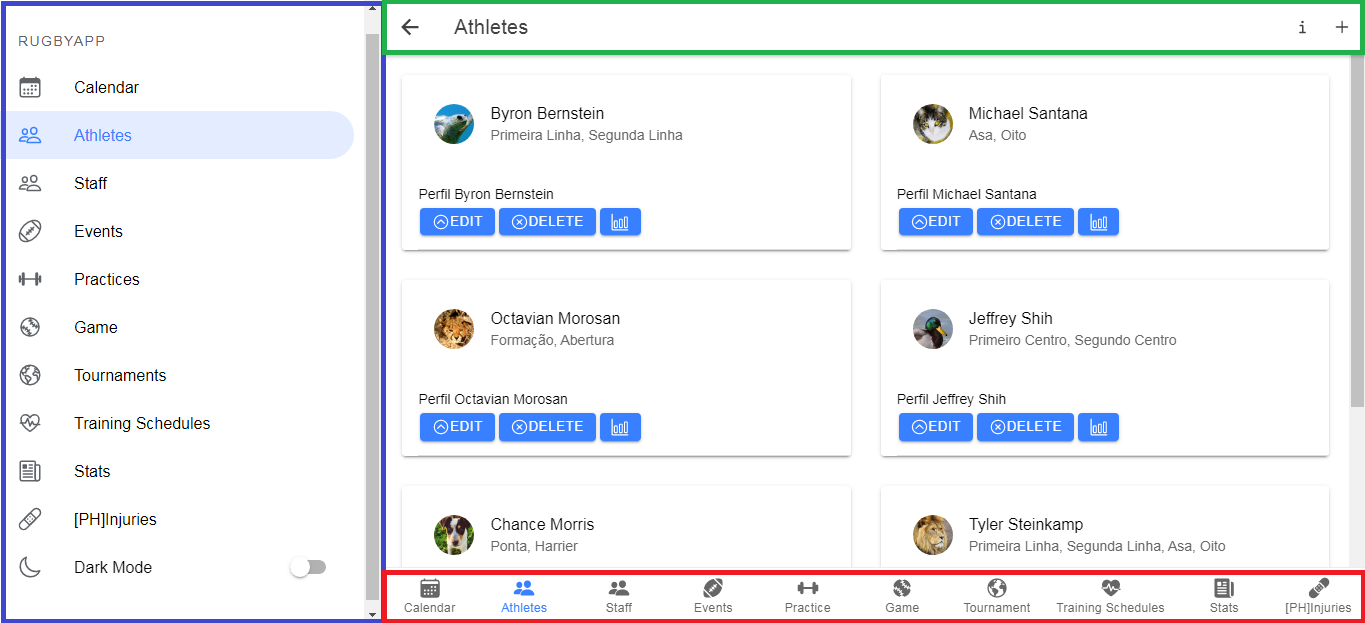
\includegraphics{./figures/frontend/MainComponent.png}}
	\end{center}
	\caption{Figura da vista inicial da aplicação. Observa-se o \textit{ion-split-pane} a azul, o \textit{ion-tabs} a vermelho e o \textit{ion-header} a verde.}\label{fig:maincomponent}
\end{figure}
\pagebreak

Como mencionado na secção 4.1.1, existem \textit{endpoints} na nossa aplicação cliente que requerem mais do que um \textit{Component} para garantir certas regras de negócios sem que a informação nas páginas fique sobrelotada e proporcionando a melhor experiência de utilização. Existem componentes na \textit{API} do \textit{Ionic} (alguns também mencionados na secção 4.1.1) que foram utilizados para este mesmo propósito\\

\begin{tabular}{ll}
	\textit{ion-modal} & \textit{Dialog} (componente visual que se sobrepõe ao contexto atual da página e \\
	&requer interação do utilizador para desaparecer), normalmente utilizado \\
	&para apresentar uma página onde o utilizador tem diversas opções de interação.\\
	& É utilizado no formulário de \textit{Practices} para o utilizador escolher na folha de \\
	&presenças os diversos tipos de treino suportados pelo nosso modelo que o \\
	&atleta realizou.\\
	\\
	\textit{ion-popover} & \textit{Dialog} (assim como o \textit{ion-modal}) que é geralmente usado para conter acções \\
	&ou informação que não pode ser mostrada na totalidade sem comprometer\\
	& visualmente os elementos da página. É utilizado nas diversas tabelas com \\
	&a lista de \textit{Events}, \textit{Games}, \textit{Tournaments}, \textit{Practices}, etc, para "esconder" a lista \\
	&de presenças atrás de um botão, para que as listas fiquem mais organizadas \\
	&e visualmente "limpas".\\
	\\
	\textit{ion-select} & Apesar de não requirir um \textit{controller} ou um \textit{component} próprio para ser \\
	&programado, o \textit{ion-select} é um \textit{ion-modal} pré-definido na \textit{API} exclusivamente \\
	&para \textit{input}/\textit{output} (ou seja, não é possível atribuir-lhe diretamente outro \\
	&comportamento que não o de dar ao utilizador diversas opções, das quais este \\
	&escolhe uma ou várias, dependendo do contexto, e o \textit{ion-select} junta-as e \\
	&guarda-as numa \textit{string}). É utilizado nos nossos formulários para dar ao \\
	&utilizador uma lista de escolhas possíveis, com que ele possa interagir para \\
	&fazer as suas escolhas.
\end{tabular}

\begin{figure}[h]
	\begin{center}
		\resizebox{150mm}{!}{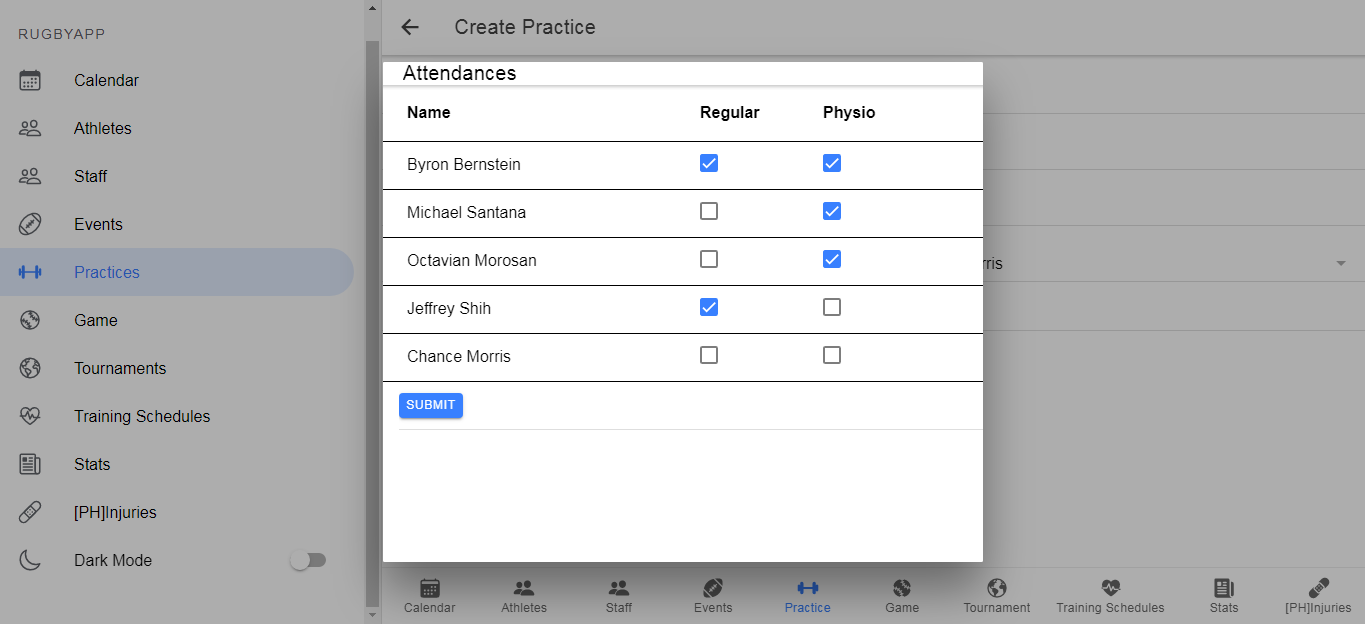
\includegraphics{./figures/frontend/PracticeFormPopover.png}}
	\end{center}
	\caption{Figura do \textit{Modal} do \textit{endpoint} do formulário de \textit{Practice}.}\label{fig:practiceformmodal}
\end{figure}
\newpage

\begin{figure}[h]
	\begin{center}
		\resizebox{150mm}{!}{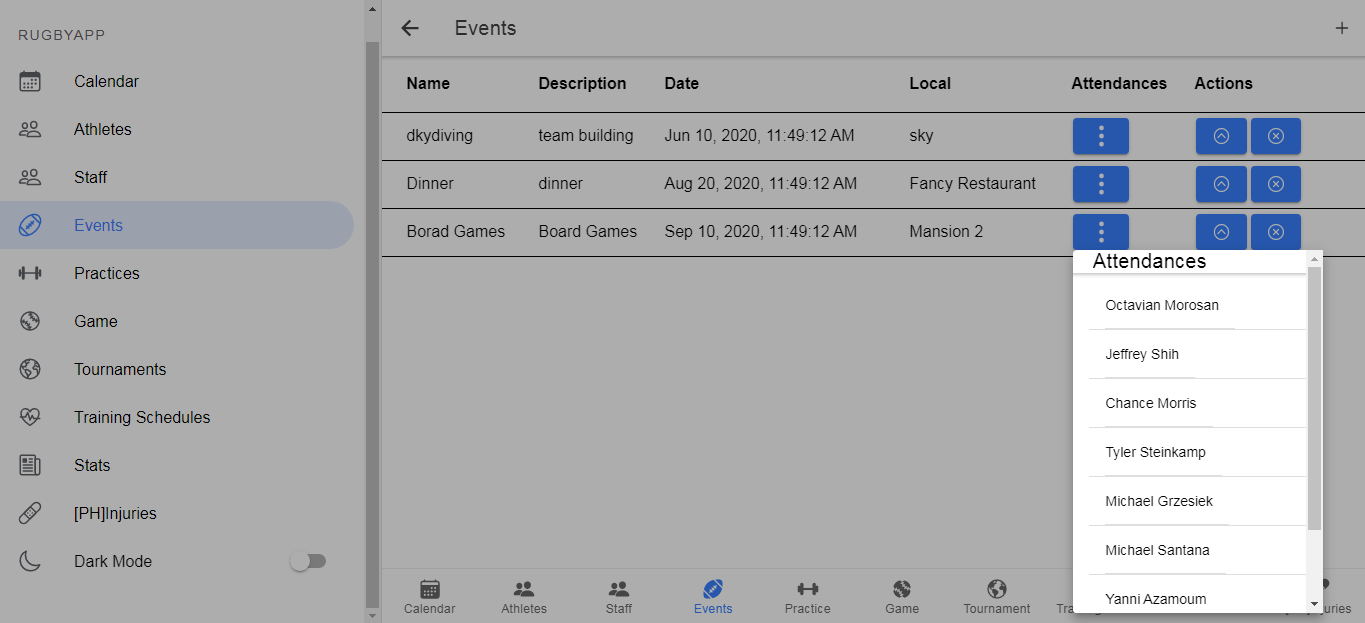
\includegraphics{./figures/frontend/EventPopover.png}}
	\end{center}
	\caption{Figura do \textit{Popover} do \textit{endpoint Event}.}\label{fig:eventpopover}
\end{figure}

\begin{figure}[h]
	\begin{center}
		\resizebox{150mm}{!}{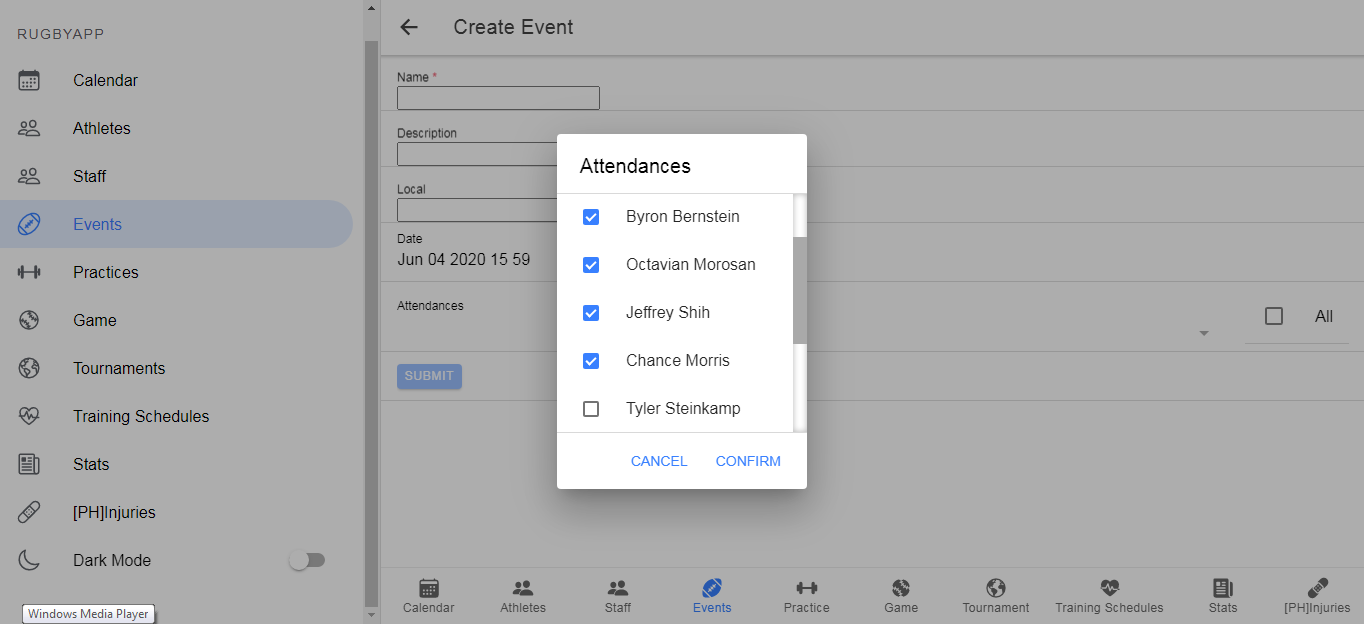
\includegraphics{./figures/frontend/EventFormSelect.png}}
	\end{center}
	\caption{Figura do \textit{Select} do \textit{endpoint} do formulário de \textit{Event}.}\label{fig:eventformselect}
\end{figure}
 \newpage
 
Como referido anteriormente, ao contrário do \textit{ion-select}, o \textit{ion-modal} e o \textit{ion-popover} são componentes próprios e requerem um \textit{controller} para serem gerados e criados por outros componentes. Podemos observar no troço de código seguinte, o método \textit{createPopover()} inserido no \textit{event.component}

\begin{lstlisting}
constructor(private eventService: EventService, private popoverController: PopoverController, private alertController: AlertController) { }

/* . . .*/

async createPopover(profiles: Profile[], ev) {
	const popover = await this.popoverController.create({
		component: EventPopoverComponent,
		componentProps: { profiles },
		event: ev
	});
	return await popover.present();
}
\end{lstlisting}



O \textit{Component event.component} importa o módulo \textit{PopoverController} do \textit{package} do \textit{Ionic}, e cria a sua instância no construtor. Atribuindo o método \textit{createPopover} a um evento, é assim invocada a criação de um \textit{Popover}. Passando esse mesmo evento ao método \textit{create} do \textit{controller}, fazemos com que o \textit{Popover} seja apresentado visualmente ligado ao botão que o criou, contrariamente a não ser passado um evento ao \textit{create}, que cria apenas um \textit{Popover} no topo da página.\\

\begin{lstlisting}
<ng-container matColumnDef="profiles">
	<th mat-header-cell *matHeaderCellDef> Attendances </th>
	<td mat-cell *matCellDef="let element">
		<ion-button (click)="createPopover(element.profiles,$event)">
			<ion-icon slot="icon-only" name="ellipsis-vertical"></ion-icon>
		</ion-button>
	</td>
</ng-container>
\end{lstlisting}



Cada elemento da coluna de \textit{Attendances} tem o seu próprio botão que vai criar o seu próprio \textit{Popover}. Passando a lista de \textit{Profiles} associadas a cada elemento, podemos criar um \textit{Popover} com cada uma das listas de \textit{Profiles} na tabela do \textit{endpoint Event}.\\

\begin{lstlisting}
<ion-header>
	<ion-title>Attendances</ion-title>
</ion-header>

<ion-content>
	<ion-list>
		<ion-item *ngFor="let profile of this.navParams.get('profiles')">
			<ng-template [ngIf]="profile.athlete" [ngIfElse]="staff">
				<ion-item detail="false" (click)="close()" routerLink="/app/athlete/athlete-profile/{{profile.id}}">
					<ion-label>
						<h3>{{profile.name}}</h3>
					</ion-label>
				</ion-item>
			</ng-template>
			<ng-template #staff>
				<ion-item detail="false" (click)="close()" routerLink="/app/staff/staff-profile/{{profile.id}}">
					<ion-label>
						<h3>{{profile.name}}</h3>
					</ion-label>
				</ion-item>
			</ng-template>
		
		</ion-item>
	</ion-list>
</ion-content>
\end{lstlisting}

Através de um módulo existente no package do \textit{Ionic}, chamado \textit{NavParams}, é possível passar informação ao \textit{Controller} do \textit{Popover}, e é possível do lado do \textit{Popover} obter essa informação para ser consumida. Neste caso, o Popover é meramente uma lista de itens com os nomes dos \textit{Profiles}, com um \textit{Link} para o \textit{endpoint} desse \textit{Profile}. É usado a terminologia \textit{ngIf} do \textit{Angular} para decidir entre gerar um \textit{Link} para o perfíl de um atleta ou de um \textit{staff}.

Do lado do \textit{ion-modal}, a ideia-chave é idêntica, exceto que o módulo que é importado pelo \textit{component} passa a ser o \textit{ModalController} em vez de \textit{PopoverController}. Continua-se a usar o \textit{NavParams} para passar informação ao \textit{Modal}, exceto que neste caso não se passa um evento para garantir que o \textit{Modal} fica visualmente ligado ao componente que o invocou, visto que o \textit{Modal} é sempre apresentado no meio da página.

\subsection{Angular Materials CDK}

O \textit{Angular} tambem dispõe de um \textit{CDK} (\textit{Component Dev Kit}) chamado \textit{Angular Materials}, onde encontramos vários componentes visuais. Em [2] podemos encontrar a lista completa de todos os componentes disponíveis neste \textit{CDK}. Apesar da nossa aplicação cliente explorar maioritariamente componentes da \textit{IONIC API}, também são usados alguns componentes deste \textit{CDK}, nomeadamente\\

\begin{tabular}{ll}
	\textit{mat-table} & Tabela usada para mostrar dados em diversos \textit{endpoints} da nossa \\
	&aplicação cliente. Esta tabela foi escolhida pelo facto de ser possível \\
	&adicionar comportamentos adicionais à tabela, como paginação, linha \\
	&de rodapé, filtro e ordenação. \\
	& \\
	\textit{mat-grid-list} & Grelha que permite variar os tamanhos que cada item ocupa na grelha,\\
	& ambos em número de colunas ou número de linhas, criando dinamismo \\
	&na organização da grelha sem a comprometer visualmente.\\
	& \\
\end{tabular}
Podemos observar no troço de código seguinte o \textit{template} da \textit{mat-table} de \textit{Games}.

\begin{lstlisting}
<ion-content>
	<table mat-table [dataSource]="this.dataSource" matSort class="mat-elevation-z8">
	
		<ng-container matColumnDef="date">
			<th mat-header-cell *matHeaderCellDef mat-sort-header> Date </th>
			<td mat-cell *matCellDef="let element"> {{element.date | date:"medium"}} </td>
		</ng-container>
		
		<ng-container matColumnDef="local">
			<th mat-header-cell *matHeaderCellDef mat-sort-header> Local </th>
			<td mat-cell *matCellDef="let element"> {{element.local}} </td>
		</ng-container>
		
		<ng-container matColumnDef="opponent">
			<th mat-header-cell *matHeaderCellDef> Opponent </th>
			<td mat-cell *matCellDef="let element">
				<ion-item>
					<ion-thumbnail slot="start"> <img [src]="element.opponent.photo"> </ion-thumbnail>
					<ion-label> {{element.opponent.name}} </ion-label>
				</ion-item>
			</td>
		</ng-container>
		
		<ng-container matColumnDef="score">
			<th mat-header-cell *matHeaderCellDef> Score </th>
			<td mat-cell *matCellDef="let element"> {{element.teamScore}} - {{element.opponentScore}} </td>
		</ng-container>
		
		<ng-container matColumnDef="comment">
			<th mat-header-cell *matHeaderCellDef> Comment </th>
			<td mat-cell *matCellDef="let element"> {{element.comment}} </td>
		</ng-container>
		
		<ng-container matColumnDef="athletes">
			<th mat-header-cell *matHeaderCellDef> Call </th>
			<td mat-cell *matCellDef="let element">
				<ion-button (click)="createPopover(element.athletes,$event)">
				<ion-icon slot="icon-only" name="ellipsis-vertical"></ion-icon>
				</ion-button>
			</td>
		</ng-container>
		
		<ng-container matColumnDef="actions">
			<th mat-header-cell *matHeaderCellDef> Actions </th>
			<td mat-cell *matCellDef="let element">
				<ion-button routerLink="/app/game/update/{{element.id}}">
					<ion-icon name="chevron-up-circle-outline"> </ion-icon>
				</ion-button>
				<ion-button (click)="presentAlert(element)">
					<ion-icon name="close-circle-outline"></ion-icon>
					</ion-button>
				<ion-button routerLink="/app/game/{{element.id}}/roster">
					<ion-icon name="person-add-outline"></ion-icon>
				</ion-button>
			</td>
		</ng-container>
		
		<tr mat-header-row *matHeaderRowDef="displayedColumns"></tr>
		<tr mat-row *matRowDef="let row; columns: displayedColumns;"></tr>
	</table>
</ion-content>
\end{lstlisting}
\newpage
As \textit{mat-table} do \textit{Angular Materials} funcionam com base num objeto \textit{DataSource}. O \textit{Component} de cada \textit{endpoint} tem uma propriedade com este objeto, e após fazer \textit{data-fetching}, afeta esta propriedade com a informação para popular a tabela com os dados. Cada \textit{Component} tem também um \textit{array} com o nome das colunas da tabela. Da forma que o \textit{mat-table} é implementado, podemos organizar os nomes neste \textit{array} com a ordem que se pretende que as colunas sejam apresentados visualmente, e a tabela será desenhada com essa ordem, independentemente da ordem como está definido o HTML de cada coluna. \\



\begin{lstlisting}
export class GameComponent implements OnInit {
	games: Game[];
	displayedColumns: string[] = ['date', 'local', 'opponent', 'score', 'comment', 'athletes', 'actions'];
	dataSource: any;
	@ViewChild (MatSort, {static: true}) sort: MatSort;

	/* . . . */

	showGames() {
		this.gameService.getGames().subscribe(games => {
			this.games = games;
			this.dataSource = new MatTableDataSource(this.games);
			this.dataSource.sort = this.sort;
		});
	}
	/* . . . */
}
\end{lstlisting}

Cada \textit{Component} também tem um \textit{decorator @ViewChild} para injetar uma referência para os elementos do \textit{template} do \textit{MatSort} nas tabelas. Afetando a propriedade \textit{sort} do nosso \textit{dataSource} para esta referência, conseguimos ativar a funcionalidade de ordenação nas nossas colunas. Como é observável no troço de código \textit{HTML} da tabela, as colunas que são ordenáveis contém o atributo \textit{mat-sort-header}. Quando a tabela é carregada na página da aplicação, ao meter o cursor por cima da coluna, se esta for ordenável, é visivél uma seta preta. Cada \textit{click} na coluna altera o estado desta seta, entre apontar para cima (a tabela está ordenada crescentemente pelos valores da coluna), apontar para baixo (a tabela está ordenada decrescentemente pelos valores da coluna) ou desaparecer (e a tabela fica organizada mediante o seu estado inicial). 
\newpage

\begin{figure}[h]
	\begin{center}
		\resizebox{150mm}{!}{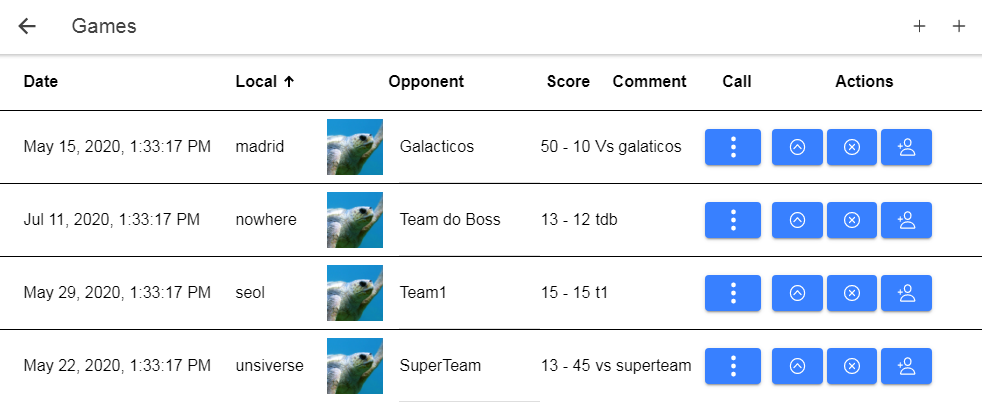
\includegraphics{./figures/frontend/GamesSortedNameUp.png}}
	\end{center}
	\caption{Figura do da tabela do \textit{endpoint} de \textit{Games}, ordenada crescentemente por nome.}\label{fig:gamessortednameup}
\end{figure}

\begin{figure}[h]
	\begin{center}
		\resizebox{150mm}{!}{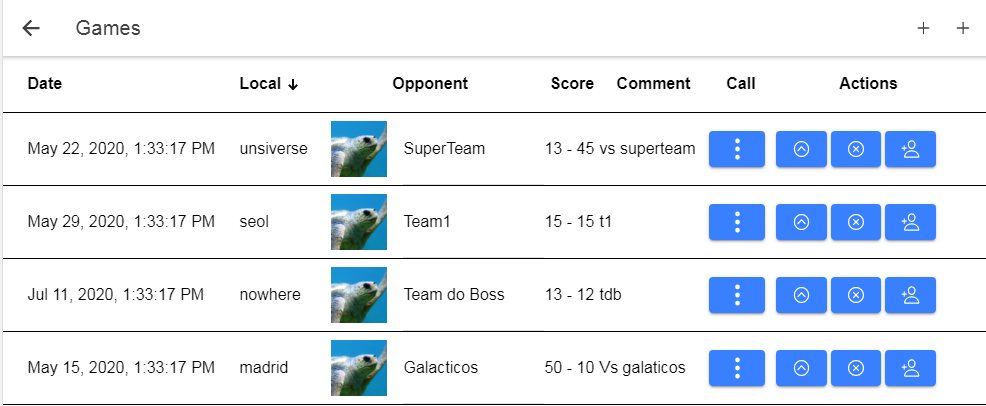
\includegraphics{./figures/frontend/GamesSortedNameDown.png}}
	\end{center}
	\caption{Figura do da tabela do \textit{endpoint} de \textit{Games}, ordenada decrescentemente por nome.}\label{fig:gamessortednameup}
\end{figure}



No que toca ao \textit{mat-grid-list}, podemos observar no troço de código seguinte como é que este componente é utilizado no \textit{Profile} de um \textit{Staff}.

\begin{lstlisting}
<mat-grid-list cols="3" rowHeight="100px">
	<mat-grid-tile [colspan]="1" [rowspan]="3">
		<img [src]="staff?.profile.photo">
	</mat-grid-tile>
	
	<mat-grid-tile [colspan]="2" [rowspan]="1">
		<ion-label>
			<div class="ion-text-center"> <b> Nome </b> </div>
			<div class="ion-text-center"> {{staff?.profile.name}} </div>
		</ion-label>
	</mat-grid-tile>
	
	<mat-grid-tile [colspan]="1" [rowspan]="1">
		<ion-label>
			<div class="ion-text-center"> <b> Tipo de Staff </b> </div>
			<div class="ion-text-center"> {{staff?.staffType.name}} </div>
		</ion-label>
	</mat-grid-tile>
	
	<mat-grid-tile [colspan]="1" [rowspan]="1">
		<ion-label>
			<div class="ion-text-center"> <b> Numero de Staff </b> </div>
			<div class="ion-text-center"> {{staff?.staffNumber}} </div>
		</ion-label>
	</mat-grid-tile>
	
	<mat-grid-tile [colspan]="1" [rowspan]="1">
		<ion-label>
			<div class="ion-text-center"> <b> Data de Nascimento </b> </div>
			<ion-datetime displayFormat="MMM DD, YYYY" value="{{staff?.profile.birth}}"></ion-datetime>
		</ion-label>
	</mat-grid-tile>
	
	<mat-grid-tile [colspan]="1" [rowspan]="1">
		<ion-label>
			<div class="ion-text-center"> <b> Morada </b> </div>
			<div class="ion-text-center"> {{staff?.profile.address}} </div>
		</ion-label>
	</mat-grid-tile>
</mat-grid-list>

\end{lstlisting}

Como referido anteriormente, uma das características chave do \textit{mat-grid-list} é a possibilidade de atribuir tamanhos diferentes aos diferentes items da grelha, permitindo-os organizar visualmente enquanto se mantem as proporções corretas da tabela. 

\begin{figure}[h]
	\begin{center}
		\resizebox{150mm}{!}{
\includegraphics{./figures/frontend/StaffProfile.png}}
	\end{center}
	\caption{Figura do \textit{Profile} de um \textit{Staff}, com as linhas da grelha \textit{highlighted} para fins de visualização. }\label{fig:calendarall}
\end{figure}

É possível aferir, com base na imagem anterior, que a grelha gerada é uma grelha 3x3, no entanto, o item da imagem do perfíl ocupa 1x3, o nome do perfíl ocupa 2x1, e os restantes itens ocupam 1x1. É possível também aferir, apesar dos tamanhos variados, que a grelha fica organizada e ocupa espaço proporcional em ambos os eixos.
\newpage

\section{Descrição dos \textit{Endpoints}}\label{sec42}

Esta secção aborda os componentes dos diversos \textit{endpoints} implementados na aplicação cliente.


\subsection{\textit{Main Component}}\label{subsec421}

O Angular gera automaticamente um \textit{root Module}, chamado \textit{AppModule}, e um \textit{AppComponent}, que servem de raiz a todos os componentes e módulos da aplicação. O nosso \textit{AppComponent} contem, como foi mencionado anteriormente e é observável na figura 4.1, um \textit{ion-split-pane} e um \textit{ion-tabs}. A instância da classe deste \textit{Component} contem um \textit{array AppPages}, onde cada objeto dentro desse \textit{array} tem um \textit{title}, um \textit{url} e um \textit{icon}, e o template deste \textit{component} gera os diferentes botões do menu através de um \textit{ngFor}. 
O \textit{ion-tabs}, por outro lado, não é diretamente implementado no \textit{AppComponent}. A nossa aplicação cliente parte o \textit{routing} em diversos componentes, sendo o principal o \textit{ion-tabs}. Foi implementado a maioria do \textit{routing} para os diversos \textit{endpoints} no \textit{ion-tabs} para garantir que em dispositivos demasiado pequenos, em termos de tamanho de \textit{ecrán}, para o \textit{ion-split-pane} ser criado, que o \textit{routing} da aplicação não seria comprometido. Por outras palavras, a entrada na aplicação dá-se, em termos de \textit{routing}, pelo \textit{ion-split-pane}, e todos os \textit{endpoints} a partir da entrada passam pelo \textit{ion-tabs}, para garantir a) que este componente é sempre criado, e b) o \textit{routing} da aplicação é sempre mantido em qualquer circunstância.
\newpage

\subsection{\textit{Calendar}}\label{subsec422}

O \textit{Calendar}, referido nesta sub-secção como Calendário, é o \textit{endpoint} principal da aplicação cliente. É a primeira página a ser mostrada quando um utilizador entra na aplicação. 

\begin{figure}[h]
	\begin{center}
		\resizebox{150mm}{!}{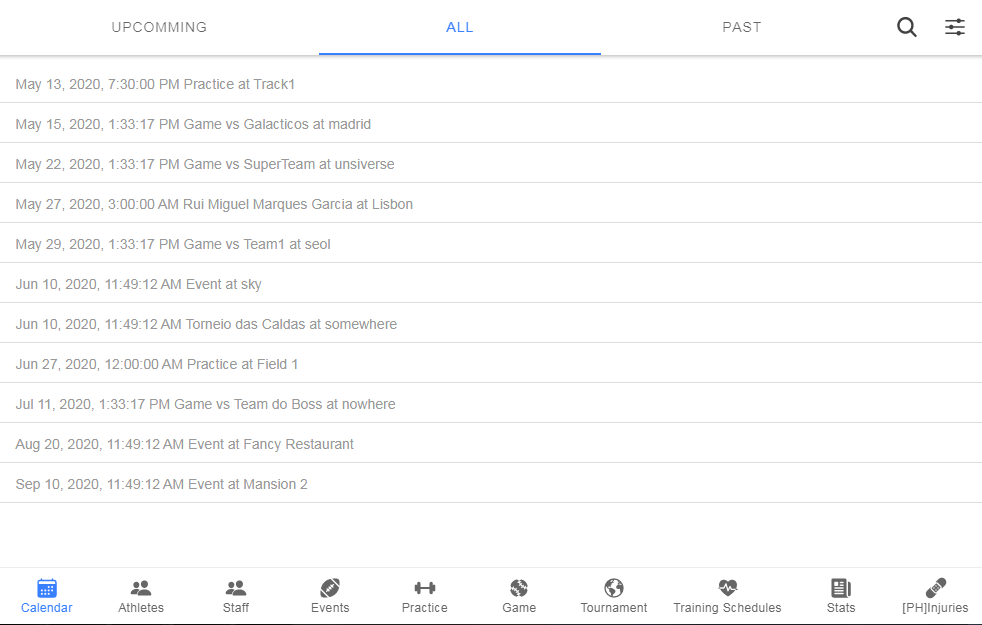
\includegraphics{./figures/frontend/CalendarAll.png}}
	\end{center}
	\caption{Figura da aba \textit{All} do Calendário.}\label{fig:calendarall}
\end{figure}

O Calendário mostra todas as entradas de \textit{Games}, \textit{Events}, \textit{Practices} e \textit{Tournaments}, através da sua data e localização.

O Calendário contem as abas \textit{Upcomming}, \textit{All} e \textit{Past}. A aba \textit{Upcomming} mostra todas as entradas que irão decorrer nos próximos N dias, sendo o valor por omissão de N 15 dias. No menu de filtro existe um campo onde é possível aumentar ou diminuir este valor de N, consoante a informação que se quer mostrar. A aba \textit{Past} mostra todas as entradas cuja data de concretização já ocorreu. A aba \textit{All} mostra todas as entradas. No caso da aba Upcomming, o calendário também mostra o tempo, em semanas, dias, horas, e minutos, até a entrada de concretização.
\newpage

\begin{figure}[h]
	\begin{center}
		\resizebox{120mm}{!}{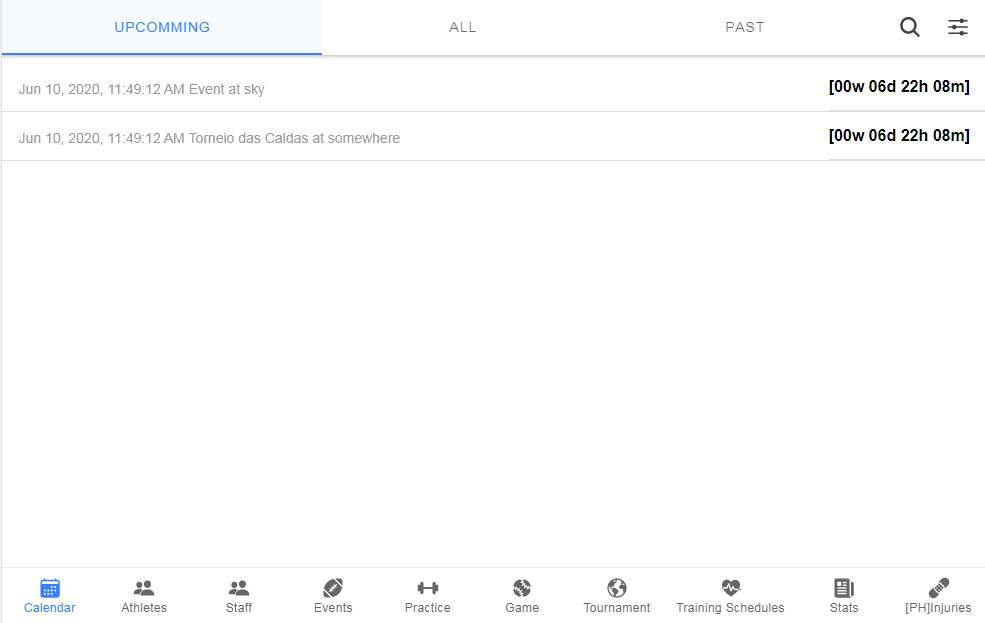
\includegraphics{./figures/frontend/CalendarUpcomming.png}}
	\end{center}
	\caption{Figura da aba \textit{Upcomming} do Calendário.}\label{fig:calendarupcomming}
\end{figure}

\begin{figure}[h]
	\begin{center}
		\resizebox{120mm}{!}{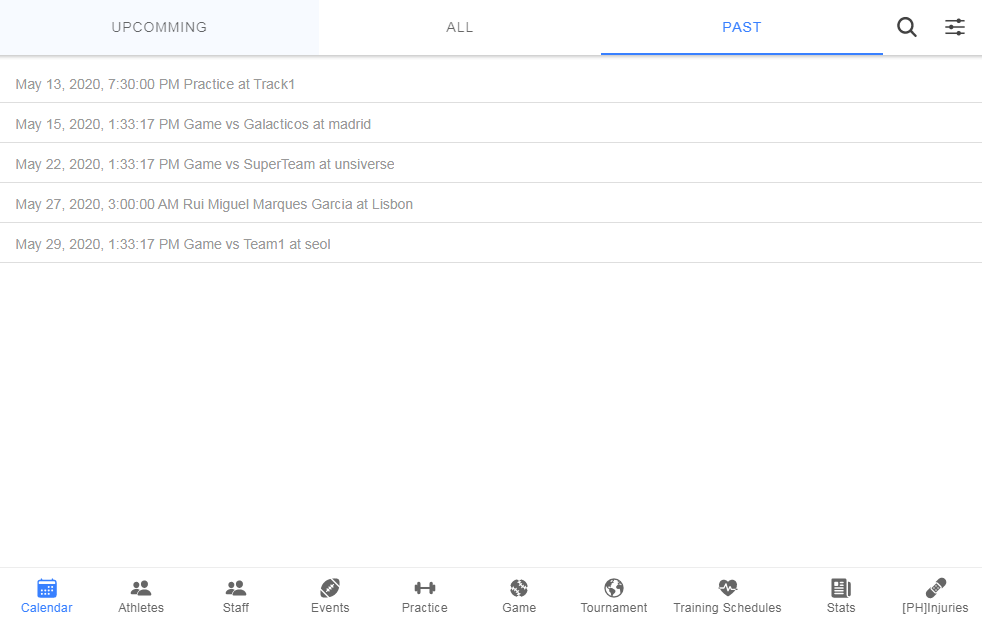
\includegraphics{./figures/frontend/CalendarPast.png}}
	\end{center}
	\caption{Figura da aba \textit{Past} do Calendário.}\label{fig:calendarpast}
\end{figure}
\newpage

O Calendário implementa uma barra de pesquisa, que pesquisa por nome, local ou oponente (caso se aplique), e apresenta apenas as entradas encontradas nessa pesquisa. Esta pesquisa é aplicada às três abas do Calendário.

\begin{figure}[h]
	\begin{center}
		\resizebox{150mm}{!}{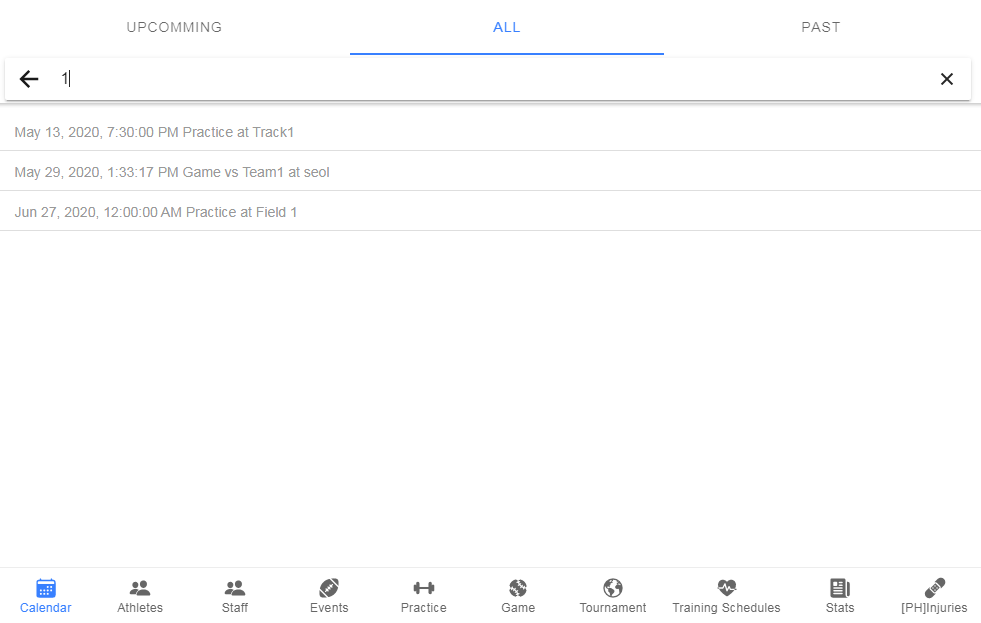
\includegraphics{./figures/frontend/CalendarSearchBar.png}}
	\end{center}
	\caption{Figura da barra de pesquisa do Calendário. A pesquisa pela \textit{string} "1" mostra todas as entradas onde o nome, local ou oponente contém essa \textit{string}. }\label{fig:gamessortednameup}
\end{figure}
\newpage

O Calendário implementa um menu de filtros, que permite filtrar por \textit{Games}, \textit{Events}, \textit{Practices} ou \textit{Tournaments}. Este filtro é aplicado às três abas do Calendário. Como referido anteriormente, tambem permite filtrar o número de dias de alcance da aba \textit{Upcomming}.

\begin{figure}[h]
	\begin{center}
		\resizebox{120mm}{!}{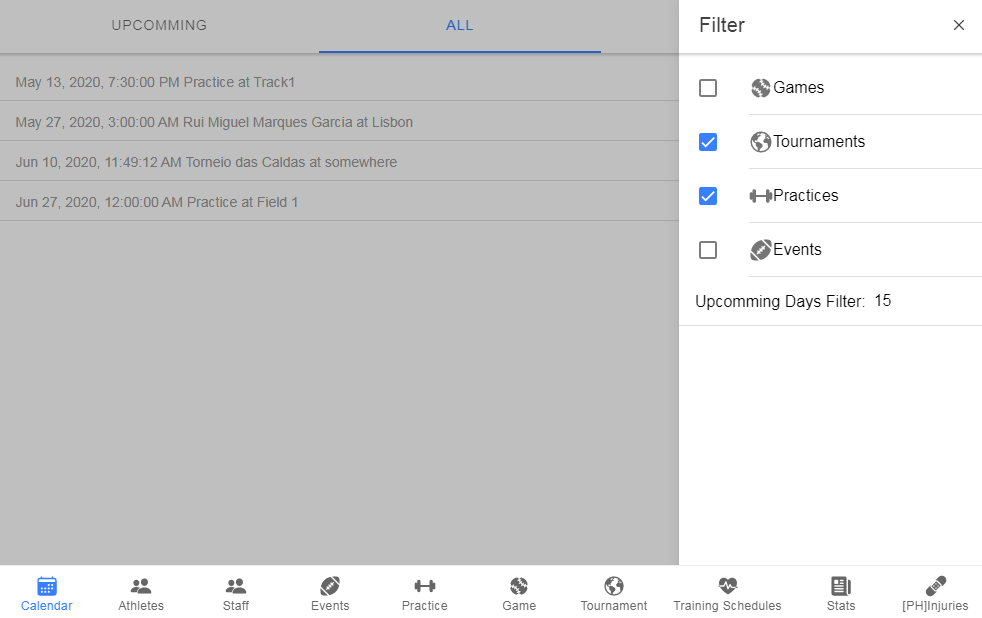
\includegraphics{./figures/frontend/CalendarFilterGamesEvents.png}}
	\end{center}
	\caption{Figura do Calendário filtrado sem \textit{Games} e \textit{Events}. }\label{fig:calendarfiltergameevents}
\end{figure}

\begin{figure}[h]
	\begin{center}
		\resizebox{120mm}{!}{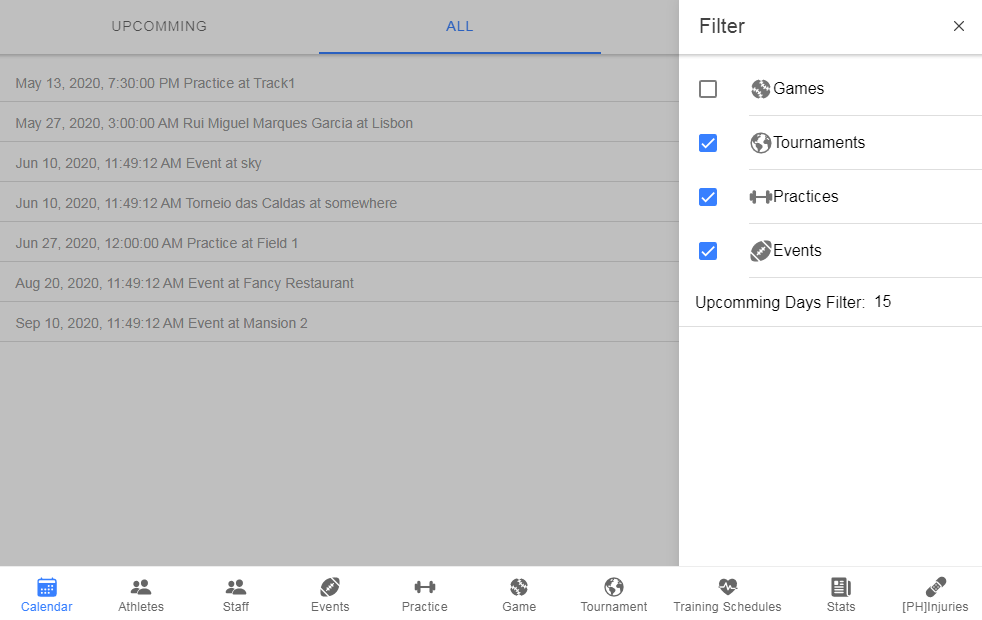
\includegraphics{./figures/frontend/CalendarFilterGames.png}}
	\end{center}
	\caption{Figura do Calendário filtrado sem \textit{Games}.}\label{fig:calendarfiltergames}
\end{figure}
\newpage

\begin{figure}[h]
	\begin{center}
		\resizebox{120mm}{!}{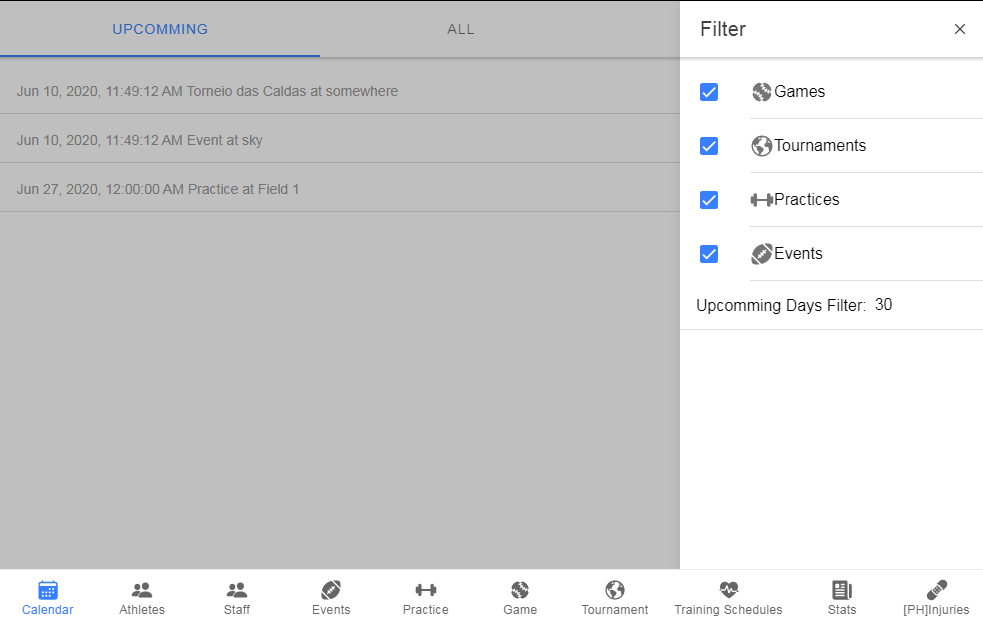
\includegraphics{./figures/frontend/CalendarFilter30Days.png}}
	\end{center}
	\caption{Figura da aba \textit{Upcomming} filtrada com 30 dias.}\label{fig:calendarfilter30days}
\end{figure}

\begin{figure}[h]
	\begin{center}
		\resizebox{120mm}{!}{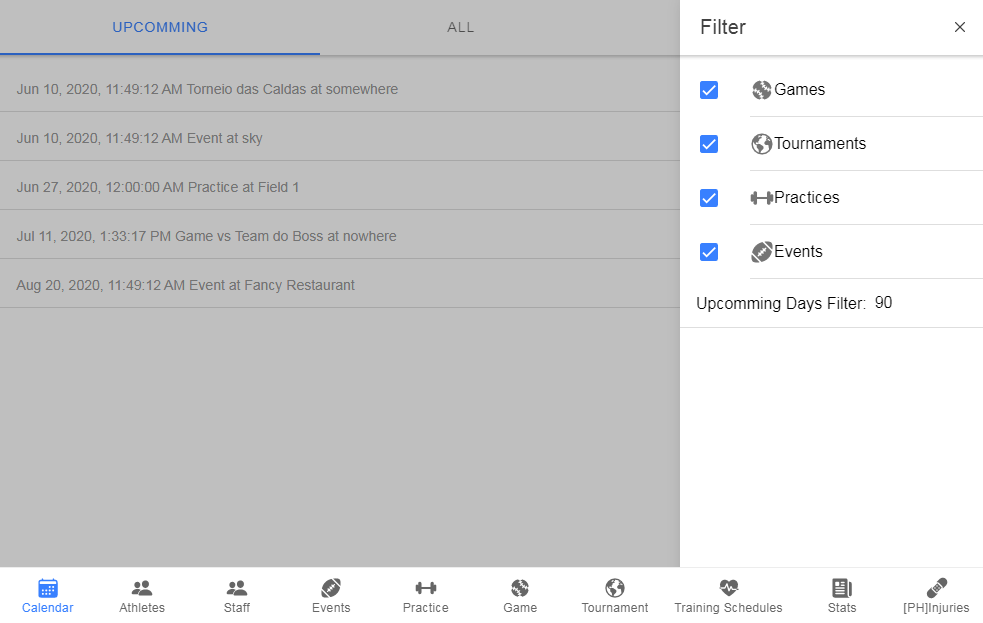
\includegraphics{./figures/frontend/CalendarFilter90Days.png}}
	\end{center}
	\caption{Figura da aba \textit{Upcomming} filtrada com 90 dias.}\label{fig:calendarfilter90days}
\end{figure}

Programáticamente, o Calendário recebe a informação através de um \textit{forkJoin}, garantido que o \textit{subscribe} do componente só é realizado quando a informação dos quatro pedidos aos quatro \textit{endpoints} da \textit{web API} da aplicação servidora forem concretizados no seu total. O Calendário contem 5 \textit{arrays} para guardar a informação que vai demonstrar, sendo estes o \textit{info}, \textit{show}, \textit{showFilter}, \textit{past} e \textit{upcomming}.

O \textit{info} é o \textit{array} que é retornado do \textit{subscribe}, que contem toda a informação agrupada num unico objeto.

O \textit{show} é uma cópia do \textit{info}, para a informação que veio da \textit{web API} não ser diretamente alterada.

O \textit{showFilter} é o \textit{array} \textit{show} filtrado com a \textit{string} adquirida da barra de pesquisa.

O \textit{past} e \textit{upcomming} agem como filtros do \textit{show}, onde um é um filtro por data com base no valor da variável \textit{upcomming\_days} (que é alterável no campo do \textit{menu} de filtro), e outro é um filtro por data com base na data corrente. Ambos são gerados através dos métodos \textit{getPast()} e \textit{getUpcomming()}. Ambos estes filtros observam o valor da barra de pesquisa, guardado numa variável \textit{searchtext}, para contextualizar se devem ser gerados a partir do \textit{show} ou do \textit{showFilter}.

O Calendário tem um método \textit{getDisplayInfo()}, que deduz através de uma variável \textit{segment} com o nome da aba que está ativa no momento, qual dos \textit{arrays} deve mostrar.

\begin{lstlisting}
export class CalendarComponent implements OnInit {
	upcomming_days = 15;
	segment = 'upcomming';
	searchtext = '';
	showSearchbar: boolean;
	info: (Event|Game|Practice|Tournament)[] = [];
	show: (Event|Game|Practice|Tournament)[] = [];
	showFilter: (Event|Game|Practice|Tournament)[] = [];
	upcomming: (Event|Game|Practice|Tournament)[] = [];
	past: (Event|Game|Practice|Tournament)[] = [];
	
	constructor(private calendarService: CalendarService, private menuController: MenuController) { }
	
	ngOnInit() {
		this.getInfo();
	}
	
	getInfo() {
		this.calendarService.getInfo().subscribe( resList => {
			this.info.push.apply(this.info, resList[0]);
			this.info.push.apply(this.info, resList[1]);
			this.info.push.apply(this.info, resList[2]);
			this.info.push.apply(this.info, resList[3]);
			this.info = this.calendarService.sortByDate(this.info);
			this.show = this.info;
			this.showFilter = this.info;
			this.getUpcomming();
			this.getPast();
		});
	}
	getPast() {
		this.past = this.searchtext ? this.calendarService.getPast(this.showFilter)
		: this.calendarService.getPast(this.show);
	}
	
	getUpcomming() {
		this.upcomming = this.searchtext ?
		this.calendarService.getUpcomming(this.showFilter,
		this.calendarService.addDays(new Date(), this.upcomming_days)) :
		this.calendarService.getUpcomming(this.show,
		this.calendarService.addDays(new Date(), this.upcomming_days));
	}
	
	getDisplayInfo() {
		if (this.segment === 'past') return this.past;
		if (this.segment === 'upcomming') return this.upcomming;
		return this.searchtext ? this.showFilter : this.show;
	}
	 /*. . .*/
}
\end{lstlisting}


Cada \textit{checkbox} do menu de \textit{filtros} está ligada a um método próprio (\textit{gameCheckChange()}, \textit{eventCheckChange()}, etc.) que faz \textit{listen} ao evento de \textit{check}/\textit{uncheck} e passa esse valor como um \textit{boolean} a um outro método de \textit{filter}(\textit{filterGame()}, \textit{filterEvent()}, etc). Este método de \textit{filter} deduz através do valor recebido se deve filtrar ou não-filtrar a informação. Exemplificando para o caso da \textit{checkbox} de \textit{Games} ser \textit{checked}, ou seja, quando a informação a mostrar deve apresentar \textit{Games}, o método chama o método filterGames() do \textit{CalendarService} sobre a \textit{info}, que vai retornar todos os \textit{Games} encontrados na informação que veio da \textit{web API} e faz \textit{push} destes \textit{Games} todos para o \textit{show}, ordenando-o prosteriormente por data. Se a mesma \textit{checkbox} for \textit{unchecked}, o método irá em vez disto chamar o método unfilterGames() do \textit{CalendarService} sobre o \textit{show}, que irá remover todas as entradas \textit{Game} deste \textit{array}. Em qualquer um dos casos, chama \textit{getPast()} e \textit{getUpcomming()} no fim para atualizar tambem os \textit{arrays} com a informação das outras abas.

\begin{lstlisting}
filterGame(bool) {
	if (bool) {
		this.show.push.apply(this.show, this.calendarService.filterGame(this.info));
		this.show = this.calendarService.sortByDate(this.show);
	}
	else this.show = this.calendarService.unfilterGame(this.show);
	this.getUpcomming();
	this.getPast();
}

gameCheckChange(e) {
	let newState = !e.currentTarget.checked;
	this.filterGame(newState);
}
\end{lstlisting}

Já a barra de pesquisa, é implementada de uma maneira menos linear. É necessário considerar, quando se faz uma pesquisa, que o utilizador pode cancelar por completo a barra de pesquisa (e a pesquisa deve ser removida), e que a cada caractere que este insere/remove, ambas as 3 abas têm de ser atualizadas com o filtro.
A barra de pesquisa está ligada a um método \textit{searchFilter()}, que é chamado cada vez que o evento da barra de pesquisa é invocado (ou seja, cada vez que o utilizador insere ou remove um caractere da pesquisa). Este método lê o valor do evento que foi invocado, e afeta a variável \textit{searchtext} com esse valor, ou com \textit{undefined} se a barra de pesquisa estiver vazia(para suplementar a lógica de que as abas \textit{Upcomming} e \textit{Past} devem filtrar o \textit{array show} em vez do \textit{array showFilter}, caso não exista pesquisa). Se existir texto na barra de pesquisa, o método invoca o \textit{searchFilter()} do \textit{CalendarService}, para filtrar o \textit{show} por texto. Este \textit{searchFilter()} filtra apenas por nome, local e/ou oponente das entradas do \textit{show}. O resultado do filtro é inserido no \textit{showFilter}. No caso da barra de pesquisa não contiver texto, o \textit{showFilter} passa apenas a ser igual ao \textit{show}. É mais uma vez chamado o \textit{getPast()} e \textit{getUpcomming()} para atualizar a informação das outras abas. Para cobrir o facto do utilizador poder simplesmente cancelar a barra de pesquisa, existe um método \textit{onCancel()} que afeta o \textit{searchtext} com \textit{undefined} e o \textit{boolean} \textit{searchBar} com \textit{false}. Depois chama o \textit{getPast()} e \textit{getUpcomming()}, que mais uma vez, como o \textit{searchtext} está a \textit{undefined}, irá filtrar pelo \textit{show} em vez de pelo \textit{showFilter}. Isto faz com que o Calendário volte ao seu estado inicial quando o utilizador cancela a barra de pesquisa.

\begin{lstlisting}
searchFilter(event) {
	this.searchtext = event.target.value.toLowerCase() === '' ? undefined : event.target.value.toLowerCase();
	if (this.searchtext) this.showFilter = this.calendarService.searchFilter(this.show, this.searchtext);
	else this.showFilter = this.show;
	this.getUpcomming();
	this.getPast();
}

onCancel() {
	this.showSearchbar = false;
	this.searchtext = undefined;
	this.getUpcomming();
	this.getPast();
	this.getDisplayInfo();
}
\end{lstlisting}

\subsection{\textit{Athletes/Staff}}\label{subsec423}

Ao contrário dos restantes componentes, o \textit{endpoint} de \textit{Athletes} e \textit{Staff} é apresentado utilizando uma listagem diferente. Foi decidido que, dado que uma lista de atletas e \textit{staff} apresenta informação que é , visualmente, mais facilmente perceptivél utilizando as fotografias dos perfís, optá-mos por fazer uma grelha com \textit{ion-cards}. Um \textit{ion-card} serve essencialmente como uma peça visual que agrupa a informação mais importante sobre um perfíl, e serve de ponto de entrada para informação mais detalhada. Podemos utilizar uma colecção de \textit{ion-cards} para agrupar toda a informação que é mais relevante numa lista de atletas sem obrigar o utilizador a entrar para dentro de um perfíl. Cada cartão tem o nome e imagem do atleta, as posições em que joga, e botões que sirvam para modificar a informação daquele atleta (\textit{edit} e \textit{delete}), assim como um botão que redireciona o utilizador para o \textit{endpoint} das estatísticas. Isto dá ao utilizador um panorâma geral dos atletas e das suas posições, com possibilidade de alterar e remover atletas da lista sem necessitar de visualizar perfís.
\newpage

\begin{figure}[h]
	\begin{center}
		\resizebox{150mm}{!}{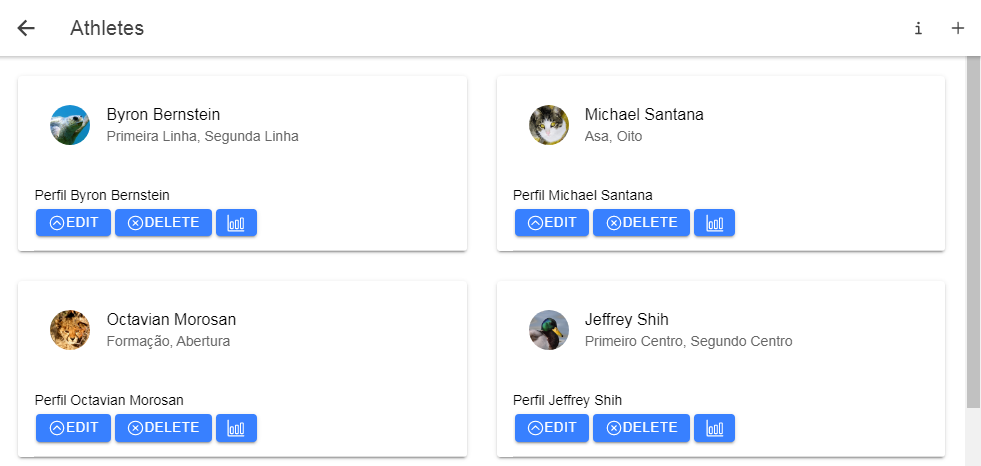
\includegraphics{./figures/frontend/AthleteList.png}}
	\end{center}
	\caption{Figura do \textit{endpoint} da lista de \textit{Athletes}.}\label{fig:athletelist}
\end{figure}

No cabeçalho deste \textit{endpoint}, são também observáveis o \textit{back button} no canto superior esquerdo, que redireciona para a página anterior, o \textit{info button} (\textbf{não implementado}) e o \textit{add button}, que redireciona para o formulário de atleta, discutido na sub-secção 4.2.8.

\subsection{\textit{Profile}}\label{subsec424}
O \textit{endpoint} de \textit{Profile} é também diferenciado dos outros \textit{endpoints} da aplicação cliente, por não mostrar uma lista de entidades, mas sim todos os dados de uma entidade específica. 
Foi decidido, como referido na sub-secção 4.1.6, usar-se uma \textit{mat-grid-list} para implementar os perfís de atletas e equipa técnica, pois a \textit{mat-grid-list} é um grelha que facilita a organização de colunas e linhas, sendo possível expandir umas e encolher outras sem comprometer visualmente a grelha. 
\newpage
\begin{figure}[h]
	\begin{center}
		\resizebox{120mm}{!}{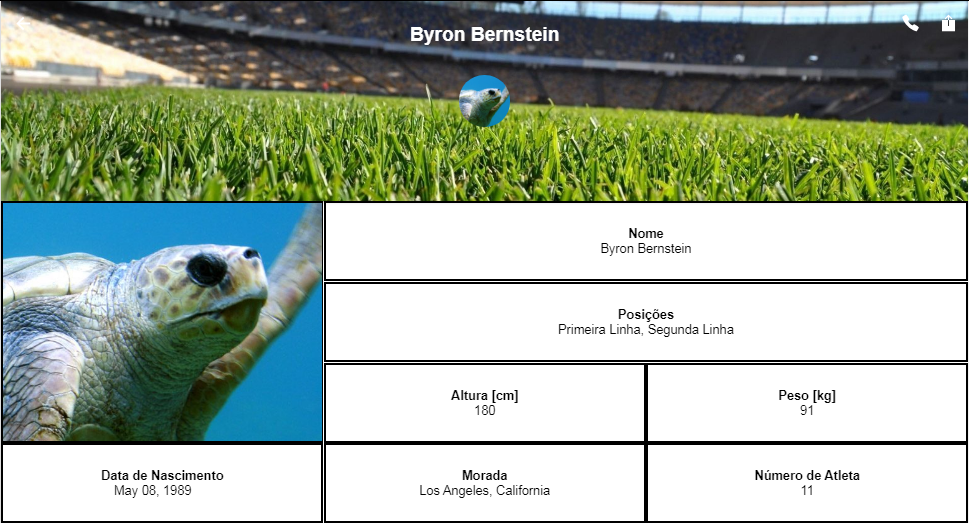
\includegraphics{./figures/frontend/AthleteProfile.png}}
	\end{center}
	\caption{Figura do \textit{endpoint} do \textit{Profile} de um \textit{Athlete}.}\label{fig:athleteprofile}
\end{figure}

O perfil de um atleta organiza assim, numa grelha 3x4, toda a informação do atleta. Também se observa, no cabeçalho do perfil, uma imagem de fundo (\textbf{irá ser alterada no futuro}), e os botões de \textit{Contact}, com o e-mail e o número de telefone do atleta para fins de entrar em contacto com este, assim como um \textit{Share} (\textbf{não implementado}).



\subsection{\textit{AthleteStats}}\label{subsec425}
O \textit{endpoint} de estatísticas de atleta é também diferenciado dos restantes \textit{endpoints} com tabelas por conter uma tabela com maior dimensão, dada a carga de dados que tem de apresentar. Neste \textit{endpoint} em particular, o \textit{split-pane} é escondido manualmente pela aplicação, para conseguir manter a tabela toda no ecrán. 

\begin{lstlisting}
ionViewDidEnter() {
	this.menuController.enable(false, 'main-menu');
}

ionViewDidLeave() {
	this.menuController.enable(true, 'main-menu');
}
\end{lstlisting}
\newpage
Para entender melhor estes métodos, é explicado em seguida o \textit{Ionic Lifecycle} de cada componente. Este \textit{lifecycle} segue a seguinte estrutura ordenada\\

\begin{tabular}{ll}
	\textit{constructor} & É executado quando a página é iniciada. É o melhor sitio \\
	&para definir valores \textit{default} para as nossas variáveis.\\
	\textit{ionViewDidLoad} & É executado quando a página foi carregada. Este evento é só \\
	&executado uma vez por cada criação de cada página. Se a página \\
	&for recarregada mas estiver em \textit{cache}, este evento não é executado\\
	& outra vez.\\
	\textit{ionViewWillEnter} & É executado quando a página está prestes a entrar e a tornar-se \\
	&a página ativa.\\
	\textit{ionViewDidEnter} & É executado quando a página entrou por completo e é agora a \\
	&página ativa. Este evento é sempre executado, independemente de \\
	&ser o primeiro carregamento da página ou se a página for \\
	&carregada da \textit{cache}.\\
	\textit{ionViewWillLeave} & É executado quando a página está prestes a sair e deixar de ser \\
	&a página ativa.\\
	\textit{ionViewDidLeave} & É executado quando a página acabou de sair e já não é a \\
	&página ativa.\\
	\textit{ionViewWillUnload} & É executado quando a página está prestes a ser destruída e os \\
	&seus elementos a serem removidos.\\
	
\end{tabular}

É possível, através deste \textit{Lifecycle}, definir quando é que alguns comportamentos são executados. Neste caso, o \textit{split-pane} é escondido no gancho \textit{ionViewDidEnter}
e volta a ser mostrado no gancho \textit{ionViewDidLeave}.

Como esta tabela contem um elevado número de colunas, foram usadas siglas para o nome de cada coluna. 

\begin{figure}[h]
	\begin{center}
		\resizebox{120mm}{!}{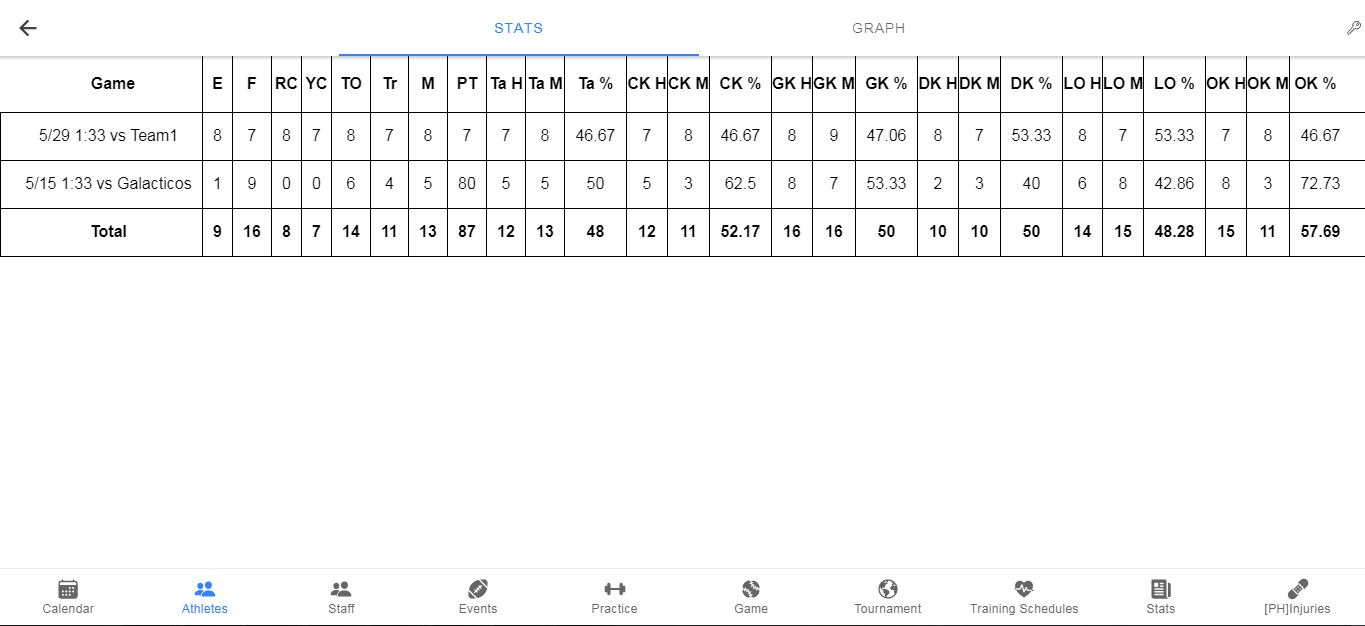
\includegraphics{./figures/frontend/AthleteStatsTable.png}}
	\end{center}
	\caption{Figura da tabela do \textit{endpoint AthleteStats}.}\label{fig:athleteprofile}
\end{figure}
\newpage

No canto superior direito do cabeçalho da página, encontramos o botão \textit{Subtitles}, que abre um menu lateral com a legenda da tabela. 

\begin{figure}[h]
	\begin{center}
		\resizebox{120mm}{!}{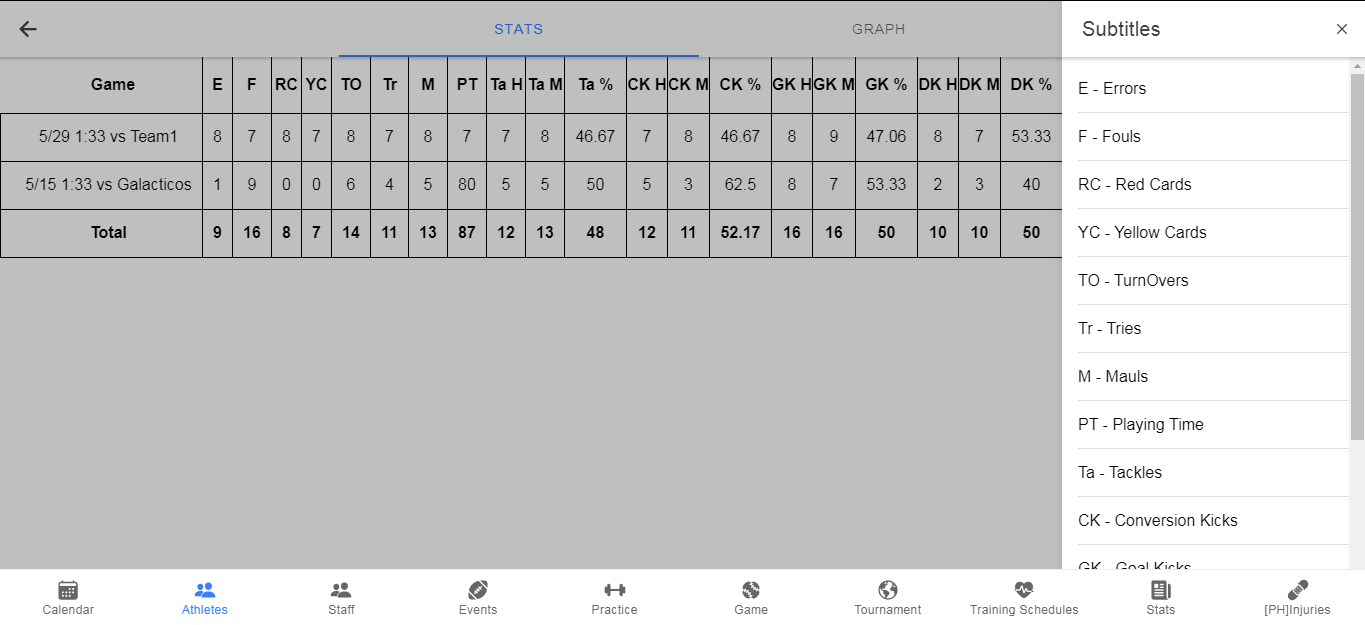
\includegraphics{./figures/frontend/AthleteStatsSubtitles.png}}
	\end{center}
	\caption{Figura da tabela do \textit{endpoint AthleteStats} com o menu da legenda aberto.}\label{fig:athleteprofile}
\end{figure}

Existe também neste \textit{endpoint} uma aba de \textit{Graphs} (\textbf{não-implementada}), que irá futuramente conter informação gráfica das estatísticas.

\subsection{\textit{Events/Practices/Games/Tournaments/TrainingSchedules}}\label{subsec426}
Estes cinco \textit{endpoints} são todos idênticos na sua estrutura, pois são os \textit{endpoints} que apresentam as tabelas das diferentes entidades.
Como foi mencionado na sub-secção 4.1.5, estes \textit{endpoints} implementam todos uma \textit{mat-table} ordenável com a informação das entidades. Dependendo do contexto das entidades, existem botões em cada linha com um \textit{Popover} com a lista de participantes/presenças/convocados, e uma coluna de Acções, onde estão os botões de \textit{Edit} e \textit{Delete}.

\begin{figure}[h]
	\begin{center}
		\resizebox{120mm}{!}{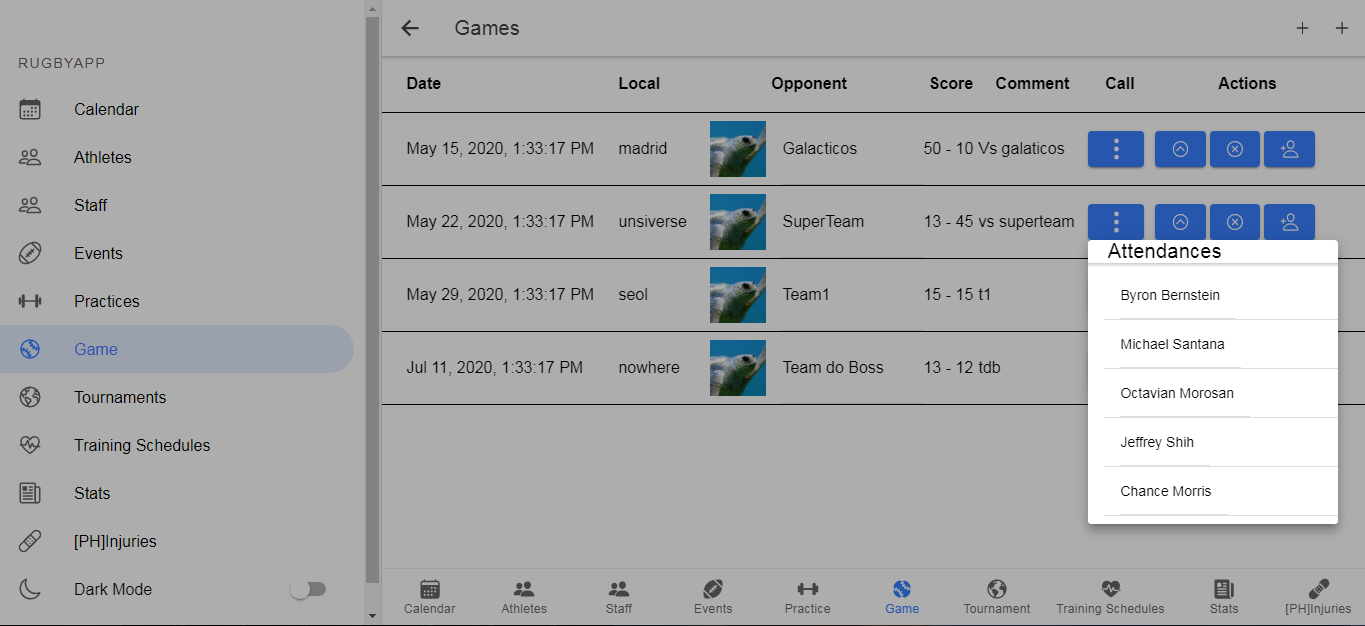
\includegraphics{./figures/frontend/GamePopover.png}}
	\end{center}
	\caption{Figura da tabela do \textit{endpoint Games}, com o \textit{Popover} aberto a mostrar os Convocados.}\label{fig:athleteprofile}
\end{figure}
\newpage
O endpoint de \textit{Games} apresenta duas diferenças distintas para todos os outros: o botão de \textit{ActiveRoster} e dois botões de \textit{Add}. 

Existem dois botões de \textit{Add} porque, como a entidade \textit{Opponent} é uma entidade fraca de \textit{Game} e não existe contextualmente sozinha com o seu próprio \textit{endpoint}, foi tomado como regra de decisão inserir o \textit{endpoint} com o formulário de adicionar um oponente no \textit{endpoint} dos jogos.

O \textit{ActiveRoster} serve para definir os titulares no contexto de um jogo. O botão de \textit{Add Active Roster} leva o utilizador para um formulário específico, onde são apresentadas as posições que os jogadores de Rugby podem cumprir, e cada posição abre um \textit{ion-select} com uma lista filtrada de atletas que jogam naquela posição.

\begin{figure}[h]
	\begin{center}
		\resizebox{120mm}{!}{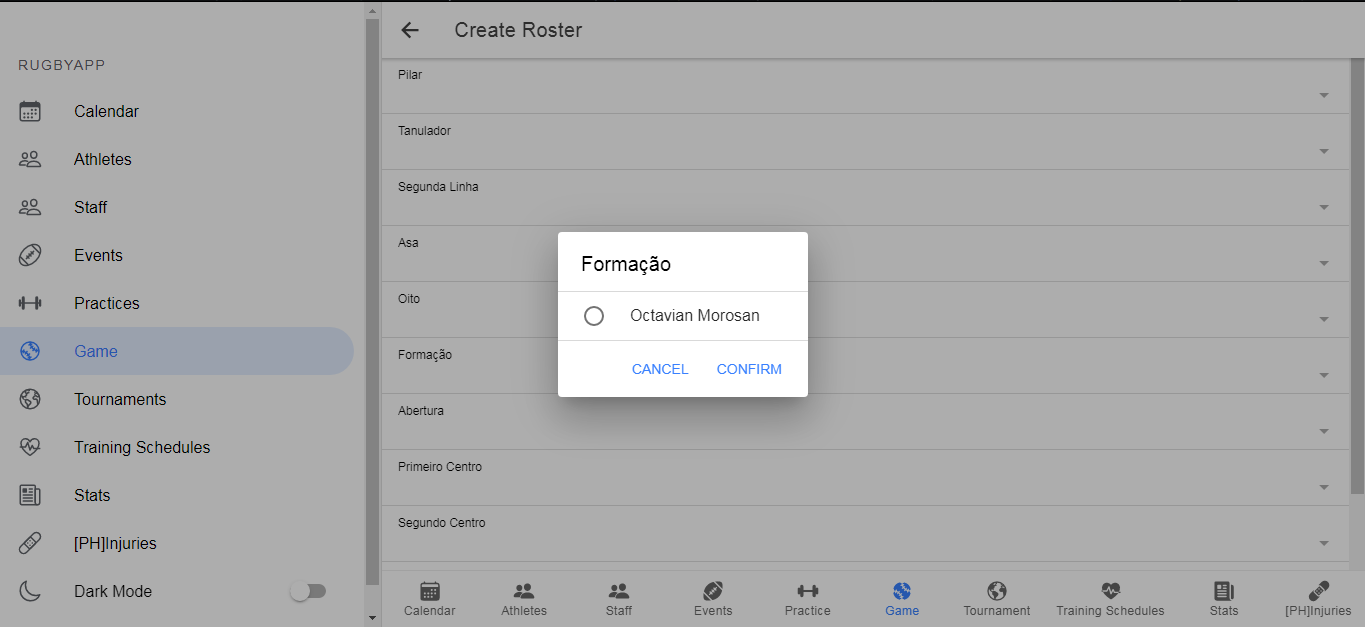
\includegraphics{./figures/frontend/ActiveRoster.png}}
	\end{center}
	\caption{Figura da tabela do \textit{endpoint ActiveRoster}, com a posição "Formação" selecionada, e o \textit{ion-select} a mostrar a lista filtrada de atletas que jogam naquela posição.}\label{fig:athleteprofile}
\end{figure}

Este formulário é implementado da seguinte maneira

\begin{lstlisting}
<form (ngSubmit)="processRoster()">
	<div *ngFor="let position of positions">
		<ion-item>
		<ion-label position="stacked"> {{position.name}} </ion-label>
		<ion-select [(ngModel)]="selected" name="selected"
		cancelText="Cancel" okText="Confirm" (ionChange)="onChange(position.id)">
			<ng-template [ngIf]="athletes != undefined">
				<ion-select-option
				*ngFor="let athlete of athleteService.getAthletesByPosition(athletes,position.name)"
				[value]="athlete">
				{{athlete.profile.name}}
				</ion-select-option>
			</ng-template>
		</ion-select>
		</ion-item>
	</div>
	<ion-item>
		<ion-button type="submit" class="ion-no-margin">Submit</ion-button>
	</ion-item>
</form>
\end{lstlisting}
\newpage

\begin{figure}[h]
	\begin{center}
		\resizebox{150mm}{!}{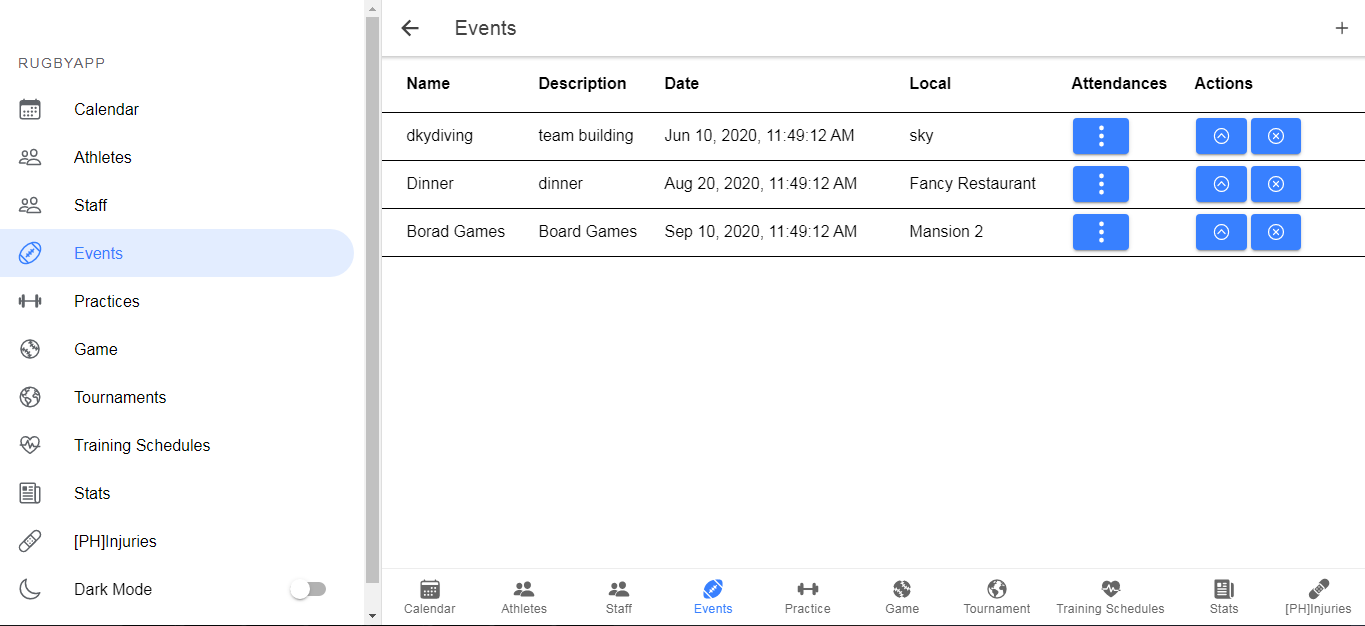
\includegraphics{./figures/frontend/Events.png}}
	\end{center}
	\caption{Figura da tabela do \textit{endpoint Events}.}\label{fig:events}
\end{figure}
\begin{figure}[h]
	\begin{center}
		\resizebox{150mm}{!}{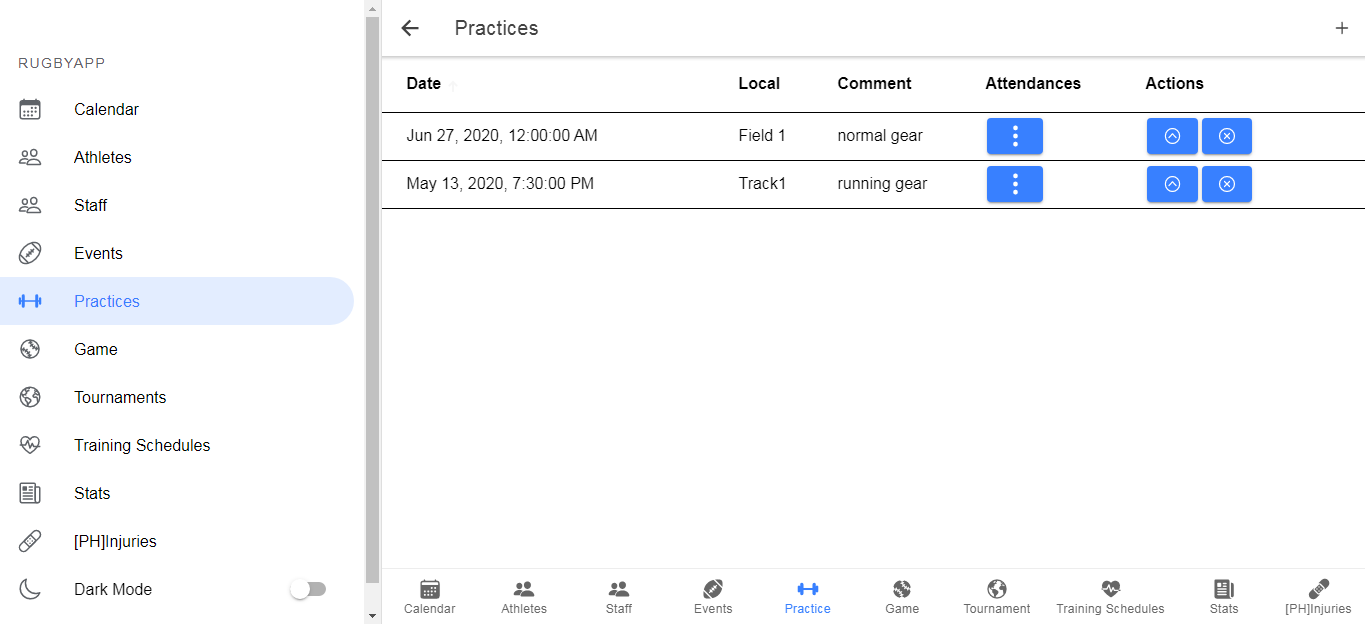
\includegraphics{./figures/frontend/Practices.png}}
	\end{center}
	\caption{Figura da tabela do \textit{endpoint Practices}.}\label{fig:practices}
\end{figure}
\newpage
\begin{figure}[h]
	\begin{center}
		\resizebox{150mm}{!}{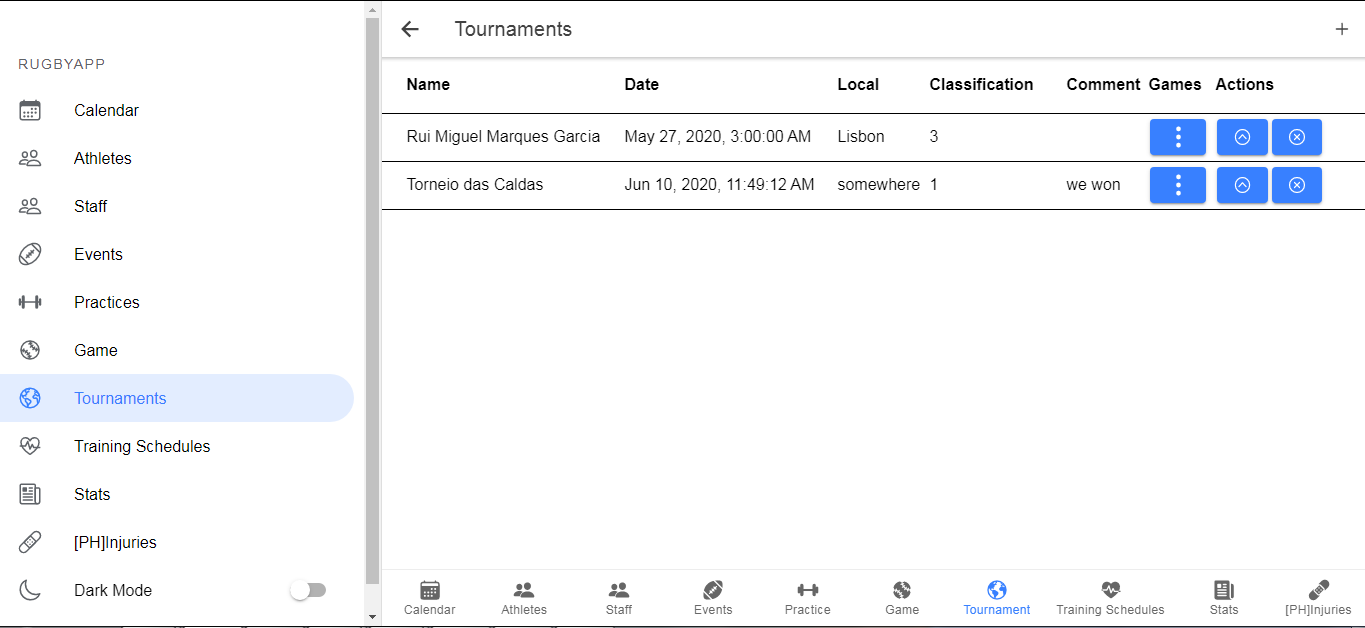
\includegraphics{./figures/frontend/Tournaments.png}}
	\end{center}
	\caption{Figura da tabela do \textit{endpoint Tournaments}.}\label{fig:tournaments}
\end{figure}
\begin{figure}[h]
	\begin{center}
		\resizebox{150mm}{!}{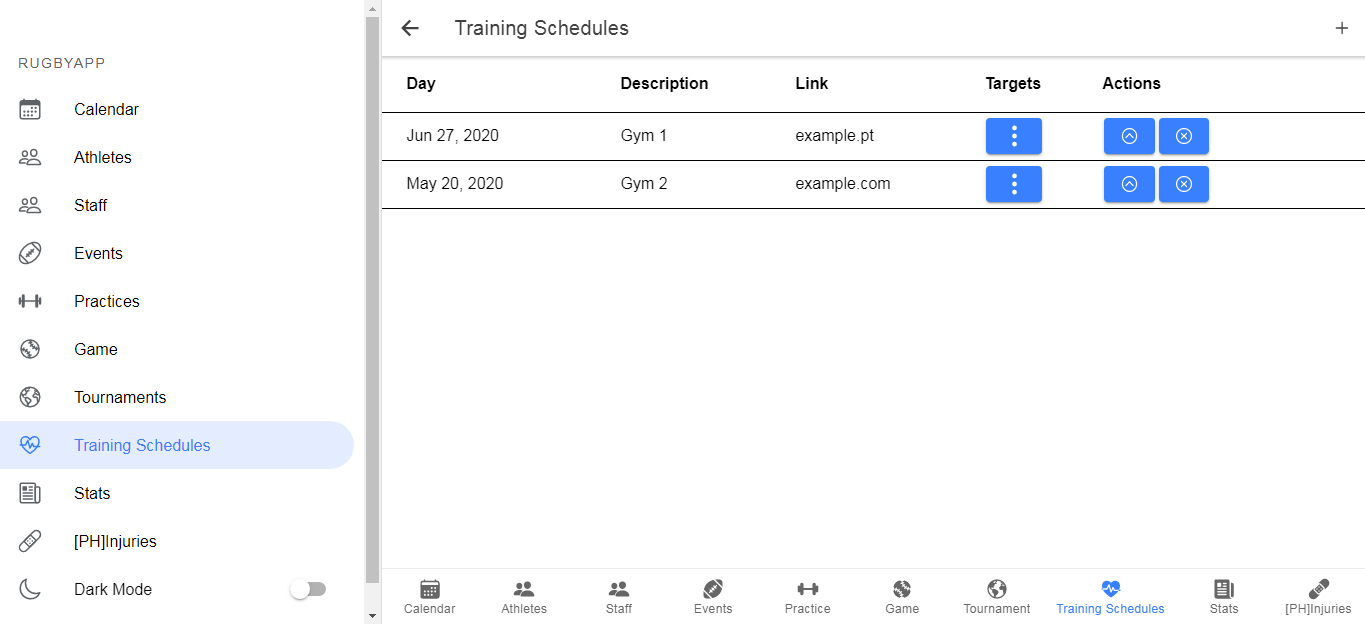
\includegraphics{./figures/frontend/TrainingSchedules.png}}
	\end{center}
	\caption{Figura da tabela do \textit{endpoint TrainingSchedules}.}\label{fig:athleteprofile}
\end{figure}
\newpage

\subsection{\textit{GameStats}}\label{subsec427}
O \textit{endpoint} de \textit{GameStats} é o endpoint principal das estatísticas de jogo. Enquanto que o \textit{AthleteStats} mostra as estatísticas associadas a um jogador, o \textit{GameStats} mostra e deixa adicionar estatísticas associadas a um jogador num jogo.

A primeira pagina deste \textit{endpoint} apresenta a lista de jogos, similarmente à lista de \textit{Athletes} ou \textit{Staff}, através duma grelha de \textit{ion-cards}. A diferença principal é que cada \textit{ion-card} encaminha para o menu de estatísticas de jogo. 

\begin{figure}[h]
	\begin{center}
		\resizebox{150mm}{!}{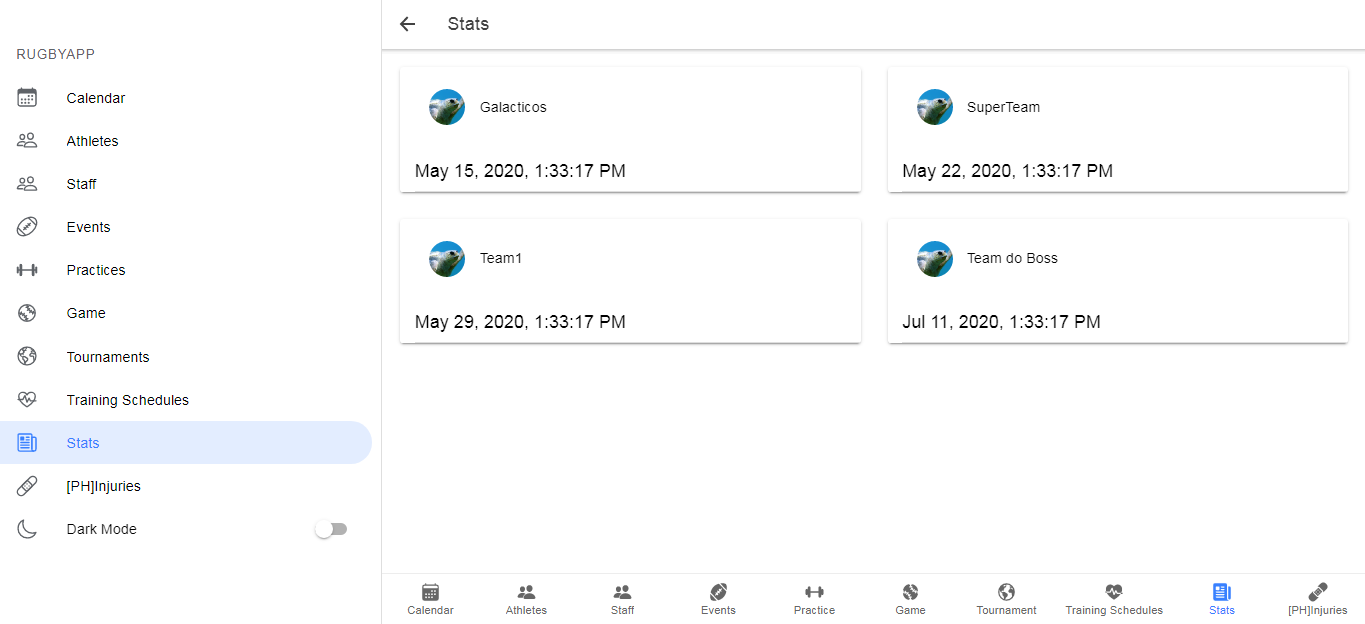
\includegraphics{./figures/frontend/StatsList.png}}
	\end{center}
	\caption{Figura da lista de \textit{Games} do \textit{endpoint GameStats}.}\label{fig:gamestatslist}
\end{figure}

O menu de estatísticas de jogo apresenta uma lista de atletas associados ao jogo em contexto (\textbf{futuramente irá só apresentar os titulares}) e permite, para cada atleta, adicionar estatísticas. 

O utilizador pode clicar em qualquer um dos atletas na lista, e este atleta é apresentado na zona de \textit{selected} como o Atleta Ativo. Todas as estatísticas do menu são atualizadas com o valor das estatísticas deste atleta, e é possivel alterá-las. As estatísticas são alteradas através de botões que incrementam o valor da estatística. No caso de estatísticas \textit{Hit} e \textit{Miss}, existem dois botões para incrementar cada um. No meio de cada item de cada estatística está o nome da estatística e o valor (no caso de \textit{Hit} e \textit{Miss} mostra ambos), e no caso também de \textit{Hit} e \textit{Miss}, encontra-se do lado esquerdo a percentagem de sucesso. Cada estatística tem também um botão de \textit{Undo} (com as \textit{Hit} e \textit{Miss} a terem dois, um para \textit{Undo} de um \textit{Hit}, outro para \textit{Undo} de um \textit{Miss}). Estes botões existem para decrementar a estatística, em caso de erro humano.
\newpage

\begin{figure}[h]
	\begin{center}
		\resizebox{120mm}{!}{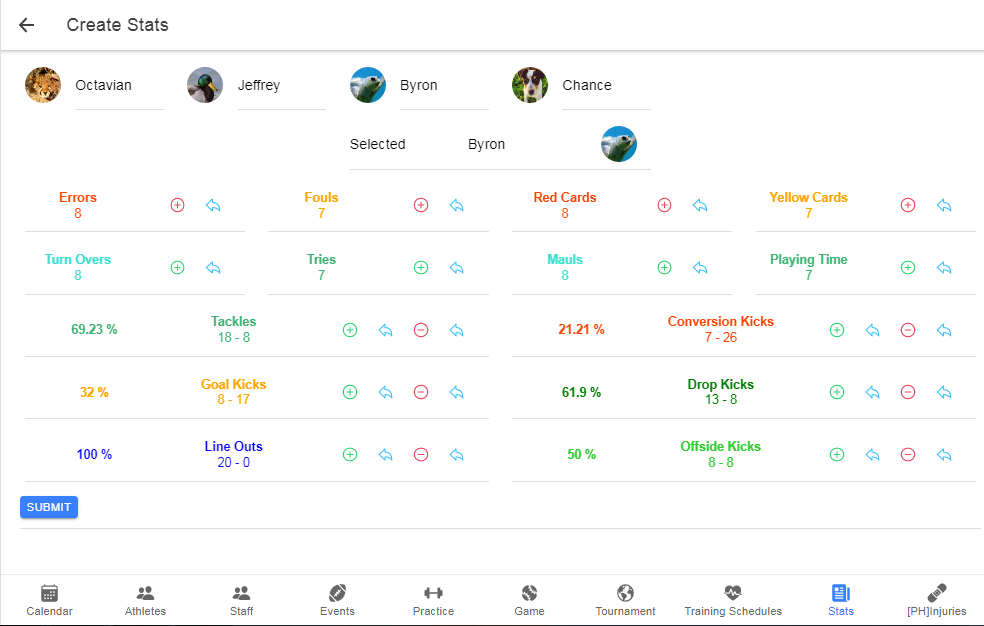
\includegraphics{./figures/frontend/GameStats2.png}}
	\end{center}
	\caption{Figura do menu de estatísticas com o atleta "Byron" selecionado.}\label{fig:gamestatslist2}
\end{figure}

\begin{figure}[h]
	\begin{center}
		\resizebox{120mm}{!}{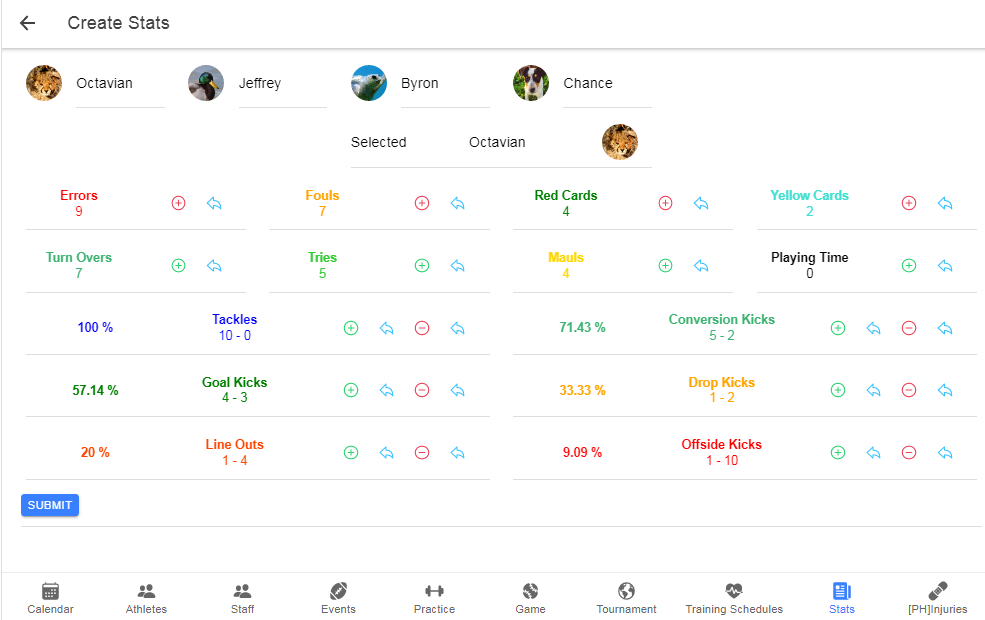
\includegraphics{./figures/frontend/GameStats.png}}
	\end{center}
	\caption{Figura do menu de estatísticas com o atleta "Octavian" selecionado.}\label{fig:gamestatslist}
\end{figure}

Este \textit{endpoint} apresenta um esquema de cores dinâmico. Como mencionado na sub-secção 4.1.3, é possível, através de um \textit{style binding}, alterar dinâmicamente o estilo de componentes \textit{HTML}. No serviço \textit{StatsService} foi definido um \textit{spectrum} (\textit{array} de \textit{strings} com valores de cores ordenados espectralmente), e cada valor de cada estatística altera a cor do texto do item para a cor indicada no \textit{spectrum}. Isto permite oferecer uma vertente visual às estatísticas de um jogador, dando uma percepção realista do seu desempenho sem considerar apenas os números. (\textbf{Este esquema está implementado estáticamente. O espectro de cores pode não corresponder à realidade de cada um, dado ser um tema emocional, e nem todos os jogos irão ter o mesmo grau de avaliação das estatísticas. Um jogo contra um oponente de nível inferior implica um maior peso negativo nos erros, e um jogo contra um oponente de nivel superior implica um menor peso negativo nos errors}).

\subsection{\textit{Forms}}\label{subsec428}
Os formulários são a principal maneira como o utilizador interage com a aplicação quando quer adicionar informação persistente (através dos \textit{endpoints} \textit{POST} ou \textit{PUT}). O formulário apresenta uma quantidade variável de campos com \textit{input} para o utilizador criar qualquer uma das Entidades. 

No contexto da aplicação cliente, o nosso \textit{endpoint} para os formulários é o mesmo para métodos de adicionar ou alterar uma entidade. No caso de o formulário ser acedido pelo \textit{update}, os campos do formulário são pré-preenchidos pelos valores atuais do objeto da entidade. Se for acedido pelo \textit{post}, os campos encontram-se vazios.
Isto concretiza-se utilizando o módulo \textit{ActivatedRoute} do \textit{Angular}, de onde é possível extrair variáveis do \textit{endpoint} que origina a criação do componente. Se o \textit{endpoint} contiver um \textit{id}, quer dizer que foi chamado no contexto de um objeto já existente, e por isso é um \textit{update} e vai, através da \textit{web API} da aplicação servidora, fazer \textit{fetch} desse objeto para pré-preencher os campos.

\begin{figure}[h]
	\begin{center}
		\resizebox{120mm}{!}{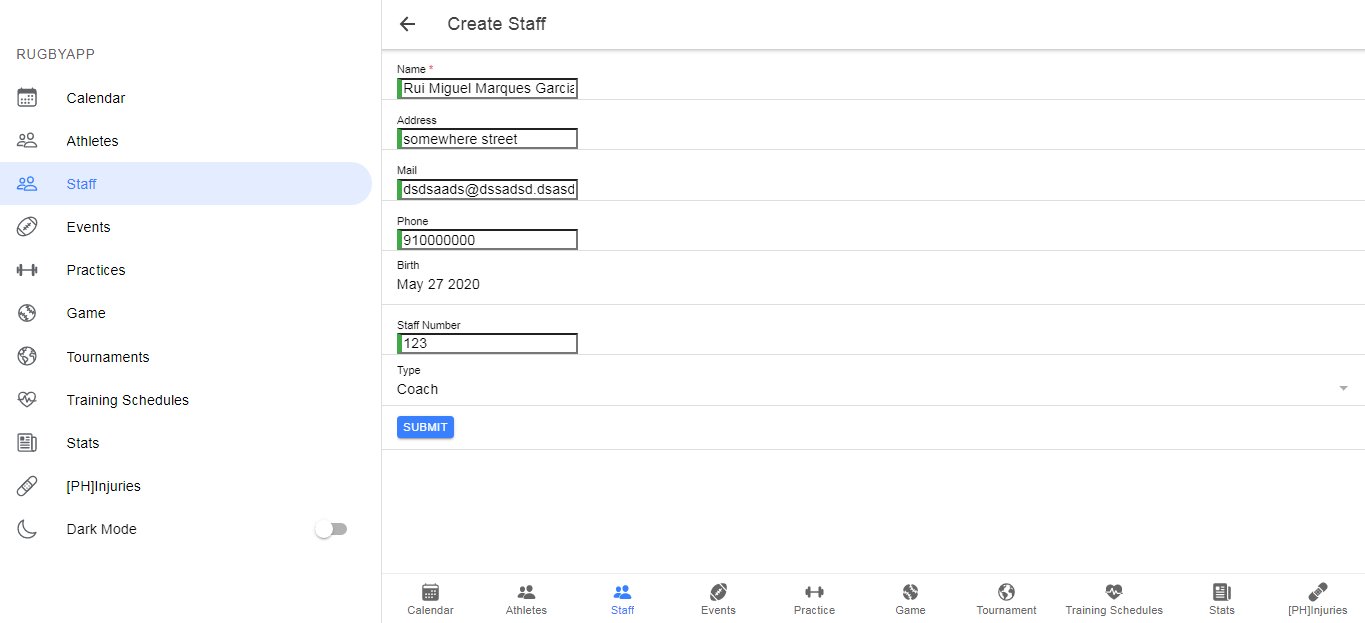
\includegraphics{./figures/frontend/FormUpdate.png}}
	\end{center}
	\caption{Figura do formulário de um \textit{Staff} quando acedido através do botão \textit{Edit} da Lista de \textit{Staff}.}\label{fig:formupdate}
\end{figure}


São utilizados alguns componentes visuais da \textit{IONIC API} para garantir uma melhor experiência de utilizador no que toca a formulários\\

\begin{tabular}{ll}
	\textit{ion-select} & Explicado em detalhe na sub-secção 4.1.4\\
	\textit{ion-datetime} & Componente visual para se escolher datas. Em vez de ser escrita \\
	&manualmente, um \textit{click} num \textit{ion-datetime} abre um menu giratório onde \\
	&o utilizador pode, através de \textit{scrolls}, escolher os valores dos diversos \\
	&campos da data. Em casos que se apliquem, como em Eventos e Jogos, \\
	&o \textit{displayFormat} da data é \textit{MMM DD AAAA HH mm} para dar a opção \\
	&de escolher a hora do evento, enquanto as datas de nascimento são em \\
	&formato \textit{MMM DD AAAA}.\\ 
	&\\
\end{tabular}

Também é possível, através dos \textit{class binding} e \textit{style binding} e \textit{attribute binding}, atribuir comportamento visual aos campos do formulário. No contexto da nossa aplicação, o botão de \textit{submit} só fica \textit{clickable} se o formulário estiver corretamente preenchido.  Através de um \textit{bind} à propriedade \textit{disabled} do botão com o objeto que representa o formulário, pode-se adicionar este comportamento ao botão, para que ele só seja \textit{enabled} quando todos os campos do formulário estão correctamente preenchidos (e só os que são \textit{required}). 

\begin{lstlisting}
<ion-item>
	<ion-button [disabled]="!loginForm.form.valid" type="submit" class="ion-no-margin">Submit</ion-button>
</ion-item>
\end{lstlisting}

Também é possível atribuir estilos \textit{html} aos campos do formulário que estão preenchidos corretamente ou incorretamente. Gerando propriedades \textit{css} para as classes \textit{.ng-valid} e \textit{.ng-invalid} que são utilizadas pelo próprio \textit{Angular} na validação de formulários, podemos ter campos bem preenchidos com uma cor verde, e os mal preenchidos com vermelho. 

\begin{lstlisting}
.ng-valid[required], .ng-valid.required {
	border-left: 5px solid #42A948;
}

.ng-invalid:not(form) {
	border-left: 5px solid #a94442;
}
\end{lstlisting}

\begin{figure}[h]
	\begin{center}
		\resizebox{120mm}{!}{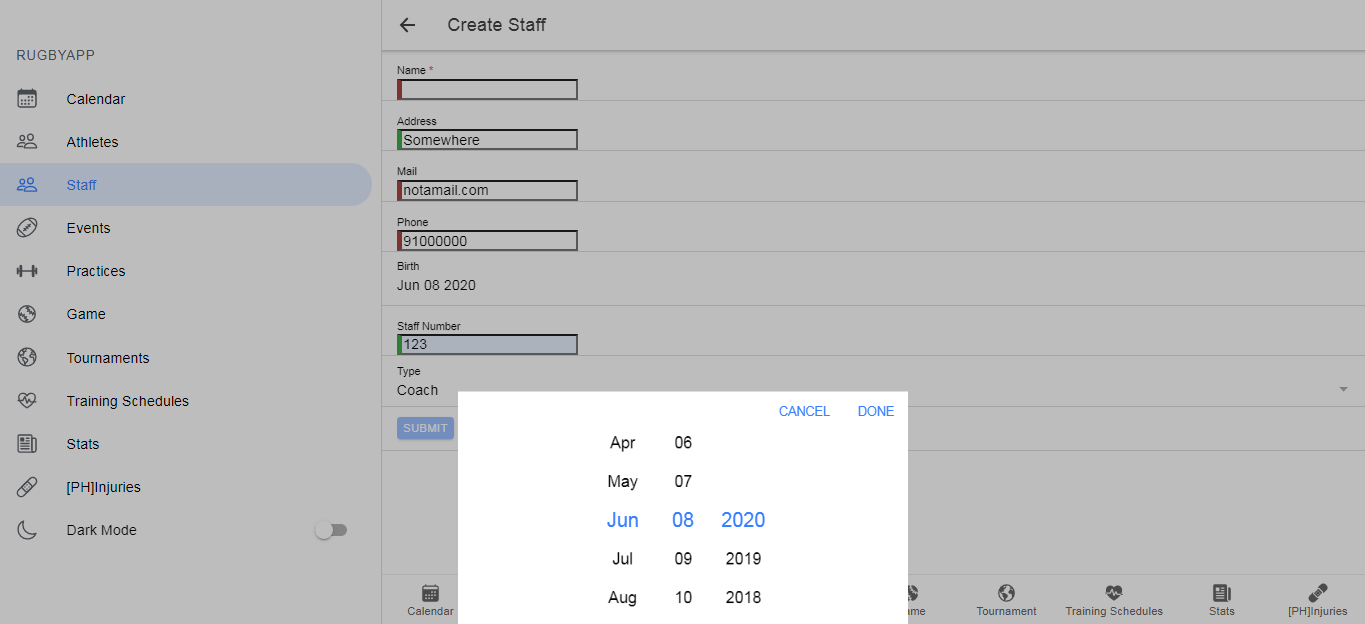
\includegraphics{./figures/frontend/FormPost.png}}
	\end{center}
	\caption{Figura do formulário de um \textit{Staff} em preenchimento.}\label{fig:formpost}
\end{figure}

Podemos observar na figura 4.30 todos os aspetos importantes de um formulário. Os campos que são \textit{required} ficam a vermelho quando não estão preenchidos, os campos que têm padrões de escrita (um número de telefone requer pelo menos 9 digitos, um e-mail requer o padrão \textit{text@text.com}) ficam a vermelho quando o padrão não é cumprido corretamente. O botão \textit{submit} encontra-se \textit{disabled} pois os campos não estão todos corretos. Ao clicar na data de nascimento, abre-se o \textit{ion-datetime}, observável também na figura.


\subsection{\textit{[WIP]Injuries}}\label{subsec428}
O \textit{endpoint} de lesões ainda não se encontra implementado. Este tema representa uma especificação funcional que foi considerada anteriormente pelos elementos do grupo como secundária. No entanto, após algumas reuniões recentes com os clubes, foi decidido aumentar a prioridade desta especificação. Apesar de não haver ainda implementação para este tema, já foi possível aferir, através de uma reunião com o fisioterapeuta do Belas Rugby Clube, o modelo da entidade \textit{Injuries}.

\begin{tabular}{ll}
	AthleteInjury&\\
	&Lesão\\
	&Situação da lesão (inicial, em recuperação, recuperado)\\
	&Data de Inicio (mais virado para organização)\\
	&Data provisória de retorno do atleta\\
	&Recomendações do fisio (exercicios para fazer em casa, precausos)\\
	&\\
	Lesão&\\
	&Nome da Lesão\\
	&Zona Corportal (orgão, osso, musculo, etc)\\
	&Severidade (há lesões iguais com graus de severidade diferentes)\\
	&\\
\end{tabular}


Futuramente, este conceito irá ser inserido na aplicação servidora junto das outras Entidades, e a aplicação cliente irá ter um \textit{endpoint} com uma lista de lesões. Possívelmente o perfíl de um atleta irá também conter alguma desta informação.
